\documentclass[11pt]{article}

\usepackage{graphicx}
\usepackage{url}
\usepackage{listings}
\usepackage{color}

\definecolor{dkgreen}{rgb}{0,0.6,0}
\definecolor{gray}{rgb}{0.5,0.5,0.5}
\definecolor{mauve}{rgb}{0.58,0,0.82}

\lstset{frame=tb,
  language=Java,
  aboveskip=3mm,
  belowskip=3mm,
  showstringspaces=false,
  columns=flexible,
  basicstyle={\small\ttfamily},
  numbers=none,
  numberstyle=\tiny\color{gray},
  keywordstyle=\color{blue},
  commentstyle=\color{dkgreen},
  stringstyle=\color{mauve},
  breaklines=true,
  breakatwhitespace=true,
  tabsize=3
}

\begin{document}

\begin{titlepage}
	\begin{center}
    	
\includegraphics[scale=0.10]{du.png}\par
		\begin{Huge}
			\textsc{University of Dhaka}\par
		\end{Huge}
		\begin{Large}
			Department of Computer Science and Engineering\par \vspace{1cm}
			CSE-3111 : Computer Networking Lab \\[12pt]	
			Lab Report 2 : Introduction to Socket Programming — Exercises on Simple Client-Server Communication.
		\end{Large}
	\end{center}  	
	\begin{large}
		\textbf{Submitted By:\\[12pt]}
			Name: Md Saim Ahmmed Utsho\\[8pt]
			Roll No : 41\\[12pt]
			Name: Md Sadmin Tahmid Khan\\[8pt]
			Roll No : 35\\[12pt]
		\textbf{Submitted On : \\[12pt]}
			February 24, 2023\\[20pt]
		\textbf{Submitted To :\\[12pt]}
			Dr. Md. Abdur Razzaque\\[12pt]
                Md Mahmudur Rahman\\[12pt]
                Md. Ashraful Islam\\[12pt]
                Md. Fahim Arefin
	\end{large}
\end{titlepage}

\section{Introduction}
Socket programming is a method of inter-process communication (IPC) that allows processes to communicate with each other over a network. Sockets provide a common interface for network communication in many operating systems, including Windows, Linux, and macOS. They can be used to create a variety of networked applications, such as client-server systems, peer-to-peer systems, and distributed systems. In socket programming, a socket is created on one process, and then connected to a socket on another process. Once connected, the processes can communicate by reading from and writing to the socket. The communication can be done using a variety of transport protocols, including TCP and UDP.

\subsection{Objectives}
The objectives of this lab experiment.
\begin{itemize}
    \item Understanding the basics of inter-process communication (IPC) and how it is used in networked applications.

    \item Learning how to create and use sockets in various programming languages, such as C, C++, Java, Python, etc.

    \item Gaining experience with the different transport protocols used in socket programming, including TCP and UDP.

    \item Developing the ability to create simple client-server systems using socket programming.

    \item Understanding the concepts of ports and sockets and how they are used in network communication.

    \item Learning how to use sockets for peer-to-peer communication and distributed systems.

    \item Understanding how to use sockets for data transfer and how to handle errors and exceptions in socket programming.

    \item Familiarizing with the best practices and guidelines of socket programming and troubleshoot common issues.

    \item Hands-on practice on various socket programming projects to understand the concepts and implementation of socket programming in real-world scenarios.
\end{itemize}
%%%%
%%%%
\section{Theory}
Inter-process communication (IPC) concept is the foundation of socket programming, as it allows processes to communicate with each other over a network. A socket is a software endpoint that allows processes to communicate with each other over a network. Sockets provide a common interface for network communication in many operating systems, including Windows, Linux, and macOS. A port is a logical endpoint for network communication on a host, and a socket is a combination of an IP address and a port. Together, they uniquely identify a network endpoint. Sockets can be used with a variety of transport protocols, including TCP and UDP. TCP is a connection-oriented protocol, which means that a connection must be established before data can be exchanged. UDP is a connectionless protocol, which means that data can be sent without first establishing a connection. Client-server systems systems involve a client process that sends requests to a server process, which responds to the requests. Client-server systems are commonly used for networked applications, such as web servers and email servers. Peer-to-peer systems involve multiple processes that can act as both clients and servers. Peer-to-peer systems are commonly used for file sharing and other decentralized applications. Error handling is an important aspect of socket programming, as it allows the programmer to handle any exceptions or errors that may occur during the execution of the program.


\section{Methodology}

\subsection{Server}
In the server side when we turn it on it will wait for any client request. If it
gets any request then it will establish a connection. Then it will read bytes from that file and send it to the client.

\subsection{Client}
On this client side, we send and receive data packets by specifying the server IP address and port number.

\section{Codes}
\subsection{Capitalize}
Client
\begin{lstlisting}
import java.io.IOException;
import java.io.ObjectInputStream;
import java.io.ObjectOutputStream;
import java.net.Socket;
import java.util.Scanner;

public class Client1a {
    public static void main(String[] args) throws IOException, ClassNotFoundException {
        System.out.println("Client Started...");
        Socket socket = new Socket("10.33.2.75", 5000);
        System.out.println("Client Connected...");

        ObjectOutputStream objectOutputStream = new ObjectOutputStream(socket.getOutputStream());
        ObjectInputStream objectInputStream = new ObjectInputStream(socket.getInputStream());

        Scanner scanner = new Scanner(System.in);
        System.out.println("Enter a sms:");
        String sms = scanner.nextLine();

        objectOutputStream.writeObject(sms);

        try {
            Object fromServer = objectInputStream.readObject();
            System.out.println("From server " + (String) fromServer);
        } catch (IOException e) {
            throw new RuntimeException(e);
        } catch (ClassNotFoundException e) {
            throw new RuntimeException(e);
        }
    }
}
\end{lstlisting}
\newpage
Server
\begin{lstlisting}
import java.net.*;
import java.io.*;

public class Server1a
{
    public static void main(String args[]) throws IOException
    {
        System.out.println("Server started");
        System.out.println("Waiting for Clients...");
        ServerSocket serverSocket = new ServerSocket(5000);

        Socket socket = serverSocket.accept();
        System.out.println("Client Accepted");
        ObjectInputStream ois = new ObjectInputStream(socket.getInputStream());
        ObjectOutputStream oos = new ObjectOutputStream(socket.getOutputStream());

        try{
            Object cMsg = ois.readObject();
            System.out.println("From Client: " + (String)cMsg);

            String serverMsg = (String) cMsg;
            serverMsg = serverMsg.toUpperCase();

            oos.writeObject(serverMsg);
        }
        catch(Exception e)
        {
            e.printStackTrace();
        }
    }
}
\end{lstlisting}
\newpage
\subsection{Prime Check}
Client
\begin{lstlisting}
import java.io.IOException;
import java.io.ObjectInputStream;
import java.io.ObjectOutputStream;
import java.net.Socket;
import java.util.Scanner;

public class Client1b {
    public static void main(String[] args) throws IOException, ClassNotFoundException {
        System.out.println("Client Started...");
        Socket socket = new Socket("10.33.2.75", 5000);
        System.out.println("Client Connected...");

        ObjectOutputStream objectOutputStream = new ObjectOutputStream(socket.getOutputStream());
        ObjectInputStream objectInputStream = new ObjectInputStream(socket.getInputStream());

        Scanner scanner = new Scanner(System.in);
        System.out.println("Enter a number to check prime:");
        int number = scanner.nextInt();

        objectOutputStream.writeObject(number);

        try {
            Object fromServer = objectInputStream.readObject();
            System.out.println("From server -> " + (String) fromServer);
        } catch (IOException e) {
            throw new RuntimeException(e);
        } catch (ClassNotFoundException e) {
            throw new RuntimeException(e);
        }
    }
}
\end{lstlisting}
\newpage
Server
\begin{lstlisting}
import java.net.*;
import java.io.*;

public class Server1b {
    public static void main(String args[]) throws IOException {
        System.out.println("Server started");
        System.out.println("Waiting for Clients...");
        ServerSocket serverSocket = new ServerSocket(5000);

        Socket socket = serverSocket.accept();
        System.out.println("Client Accepted");
        ObjectInputStream ois = new ObjectInputStream(socket.getInputStream());
        ObjectOutputStream oos = new ObjectOutputStream(socket.getOutputStream());

        try {
            Object cMsg = ois.readObject();
            System.out.println("From Client: " + (int) cMsg);

            int serverMsg = (int) cMsg;

            boolean ans = isPrime(serverMsg);

            if (ans == true)
                oos.writeObject("The number is prime");
            else
                oos.writeObject("The number is not prime");
        } catch (Exception e) {
            e.printStackTrace();
        }
    }
    static boolean isPrime(int num) {
        if (num <= 1) {
            return false;
        }
        for (int i = 2; i <= num / 2; i++) {
            if ((num % i) == 0)
                return false;
        }
        return true;
    }
}

\end{lstlisting}
\newpage
\subsection{ATM}
Client
\begin{lstlisting}
import java.io.*;
import java.lang.Math;
import java.net.Socket;
import java.util.*;;

public class Client2 {
    public static void main(String[] args) throws IOException, ClassNotFoundException {
        delay();
        System.out.println("Client Started...");
        // Socket socket = new Socket("10.33.2.75", 5000);

        Socket socket = new Socket("localhost", 5000);

        Scanner scanner = new Scanner(System.in);
        delay();
        System.out.println("Client Connected...");
        delay();
        System.out.println("Enter your username:");
        String name = scanner.nextLine();
        delay();
        System.out.println("Enter your password:");
        String pass = scanner.nextLine();

        ObjectOutputStream objectOutputStream = new ObjectOutputStream(socket.getOutputStream());
        ObjectInputStream objectInputStream = new ObjectInputStream(socket.getInputStream());

        objectOutputStream.writeObject(name);
        objectOutputStream.writeObject(pass);

        Object fromServer1 = objectInputStream.readObject();

        if ((boolean) fromServer1 == true) {
            delay();
            System.out.println("\nLogin Successful...");

            String str;
            int val;

            while (true) {

                delay();

                System.out.println("\nChoose Option please:\n");
                System.out.println("Press b to check balance");
                System.out.println("Press c to Credit balance");
                System.out.println("Press d to Debit balance");
                System.out.println("Press q to Log Out\n");

                str = scanner.nextLine();
                objectOutputStream.writeObject(str);

                sendPackets();

                if (str.equals("q")) {
                    delay();
                    Object fromServer = objectInputStream.readObject();
                    System.out.println("\n" + fromServer);

                    break;
                }
                try {
                    delay();
                    Object fromServer = objectInputStream.readObject();
                    System.out.println("\n" + fromServer);

                    if (str.equals("c") || str.equals("d")) {

                        val = scanner.nextInt();
                        scanner.nextLine();

                        int loop = req_error();

                        objectOutputStream.writeObject(loop);

                        for (int i = 0; i < loop; i++) {

                            String time = "";

                            if (i == 0)
                                time = "once...";
                            else if (i == 1)
                                time = "twice...";

                            System.out.println("\nSending data packets " + time);
                            delay();

                            objectOutputStream.writeObject(val);

                            sendPackets();
                        }
                        try {
                            Object fromServer2 = objectInputStream.readObject();
                            delay();
                            System.out.println("\n" + fromServer2);
                        } catch (Exception e) {
                            e.printStackTrace();
                        }
                    }

                } catch (Exception e) {
                    e.printStackTrace();
                }
            }
        }

        else {
            delay();
            System.out.println("Login Failed! Try again...");
            System.exit(0);
        }
    }

    static int req_error() {
        return (int) Math.floor(Math.random() * (2)) + 1;
    }

    static boolean error() {

        int num = (int) Math.floor(Math.random() * (100));

        if (num < 70) {
            delay();
            System.out.println("\nData packets sent successfully to the Server...\n");
            return true;
        } else {
            delay();
            System.out.println("\nData packets not sent to the server\nResending packets...\n");
            return false;
        }
    }

    static void sendPackets() {
        while (true) {
            if (error() == true)
                break;
        }
    }

    static void delay() {
        try {
            Thread.sleep(1000);
        } catch (InterruptedException e) {
            e.printStackTrace();
        }
    }

}
\end{lstlisting}
\newpage
Server
\begin{lstlisting}
import java.net.*;
import java.io.*;
import java.util.*;

public class Server2 {
    String user;
    String password;
    int balance;

    Server2(String user, String password, int balance) {
        this.user = user;
        this.password = password;
        this.balance = balance;
    }

    public void setBalance(int newBalance) {
        this.balance = newBalance;
    }

    public int getBalance() {
        return this.balance;
    }

    public String checkBalance() {
        return "Your current balance is: " + getBalance() + " taka";
    }

    public void credit(int value) {
        setBalance(getBalance() + value);
    }

    public boolean debit(int value) {
        if (getBalance() >= value) {
            setBalance(getBalance() - value);
            return true;
        } else
            return false;
    }

    public static void main(String args[]) throws IOException {
        int userNo = -1;

        Server2[] users;

        users = new Server2[3];

        users[0] = new Server2("Rahim", "1234", 50000);
        users[1] = new Server2("Karim", "1234", 60000);
        users[2] = new Server2("Rafiq", "1234", 40000);

        delay();

        System.out.println("Server started");

        delay();

        System.out.println("Waiting for Clients...");

        ServerSocket serverSocket = new ServerSocket(5000);
        Socket socket = serverSocket.accept();
        delay();
        System.out.println("Client Accepted");
        ObjectInputStream ois = new ObjectInputStream(socket.getInputStream());
        ObjectOutputStream oos = new ObjectOutputStream(socket.getOutputStream());

        try {
            Object cMsg1 = ois.readObject();
            Object cMsg2 = ois.readObject();

            String Name = (String) cMsg1;
            String Pass = (String) cMsg2;

            for (int i = 0; i < 3; i++) {
                if (Name.equals(users[i].user) && Pass.equals(users[i].password)) {
                    oos.writeObject(true);
                    userNo = i;
                    break;
                } else
                    oos.writeObject(false);
            }
            while (true) {
                Object cMsg3 = ois.readObject();
                String command = (String) cMsg3;

                if (userNo >= 0) {
                    if (command.equals("c")) {

                        sendPackets();

                        oos.writeObject("Enter amount to be credited:\n");

                        Object cMsg4 = ois.readObject();
                        int loop = (int) cMsg4;

                        if (loop == 1) {
                            Object cMsg5 = ois.readObject();
                            int value = (int) cMsg5;

                            users[userNo].credit(value);

                            sendPackets();

                            oos.writeObject("Your account has been credited by " + value + " taka\n"
                                    + users[userNo].checkBalance());
                        } else if (loop == 2) {
                            Object cMsg5 = ois.readObject();
                            int value = (int) cMsg5;

                            Object cMsg6 = ois.readObject();
                            int value1 = (int) cMsg6;

                            users[userNo].credit(value);

                            sendPackets();

                            oos.writeObject("Your account has been credited by " + value + " taka\n"
                                    + users[userNo].checkBalance());
                        }

                    } else if (command.equals("d")) {

                        sendPackets();

                        oos.writeObject("Enter amount to be debited:\n");

                        Object cMsg4 = ois.readObject();
                        int loop = (int) cMsg4;

                        if (loop == 1) {
                            Object cMsg5 = ois.readObject();
                            int value = (int) cMsg5;

                            sendPackets();

                            if (users[userNo].debit(value) == true)
                                oos.writeObject("Your account has been debited by " + value + " taka\n"
                                        + users[userNo].checkBalance());
                            else
                                oos.writeObject("Insufficient Balance\n" + users[userNo].checkBalance());

                        } else if (loop == 2) {
                            Object cMsg5 = ois.readObject();
                            int value = (int) cMsg5;

                            Object cMsg6 = ois.readObject();
                            int value1 = (int) cMsg6;

                            sendPackets();

                            if (users[userNo].debit(value) == true)
                                oos.writeObject("Your account has been debited by " + value + " taka\n"
                                        + users[userNo].checkBalance());
                            else
                                oos.writeObject("Insufficient Balance\n" + users[userNo].checkBalance());
                        }
                    } else if (command.equals("q")) {

                        sendPackets();

                        oos.writeObject("Log Out Successful...\n");

                        delay();

                        System.out.println("System shutting down...\n");

                        break;
                    } else if (command.equals("b")) {

                        sendPackets();

                        oos.writeObject(users[userNo].checkBalance());
                    }
                }
            }
        } catch (Exception e) {
            e.printStackTrace();
        }
    }
    static boolean error() {

        int num = (int) Math.floor(Math.random() * (100));

        if (num < 70) {
            delay();
            System.out.println("\nData packets sent successfully to the Client...\n");
            return true;
        } else {
            delay();
            System.out.println("\nData packets not sent to the Client\nResending packets...\n");
            return false;
        }
    }
    static void sendPackets() {
        while (true) {
            if (error() == true)
                break;
        }
    }
    static void delay() {
        try {
            Thread.sleep(1000);
        } catch (InterruptedException e) {
            e.printStackTrace();
        }
    }
}
\end{lstlisting}
\section{Code Explanation}
\begin{enumerate}
    \item \textbf {ATM user login:} We used an array of objects of Users. The object user has 3 variables - name, password and balance. We created 3 users - Rahim, Karim and Rafiq.
    \item \textbf {User request:} In our system, we used class that consists of set and get methods for a user's balance. Moreover, we used methods for checking balance, crediting and debiting using get and set methods.
    \item \textbf {Handling errors:} In our ATM system, we are running both the server and the client side PCs next to each other. Hence, the chance of unsuccessful data transmission between client and server is very low, given that the codes are correct. However, in real world applications, the server and the clients may be very far from each other, which may give rise to errors while transmitting data. In our system we tried to introduce errors by random function. We created a boolean function -  error() in both the client and server side. Here a number is generated in random from 1 - 100. If the number generated is greater than 70, we assume the packets being sent have been unsuccessful and if the number is less than 70, the data packets being sent are assumed to be unsuccessful. Before sending a packet from client to server or from server to client, we send the packets by using a while loop. Here, the data packets will be sent only when there is no error (random number generates more than 70). The data is received only when there are no errors while sending.
    \item \textbf {Handling idempotent operations:} In an ATM system it is not possible that a user’s account is credited twice instead of once by mistake. In our system we included a method such that the same operation when requested twice or more times is carried out only once; we handled the request automatically. We included a method where a request can be either sent once or twice; the number of times the request is being sent is determined using a random value between one and two. The request will be processed once, regardless of the number of requests incoming. As a result the system is made to handle idempotent operation.
\end{enumerate}




\newpage


\section{Experimental result}

Some Snapshots can be seen in the following figures: 

\begin{figure}[!h]
\centering
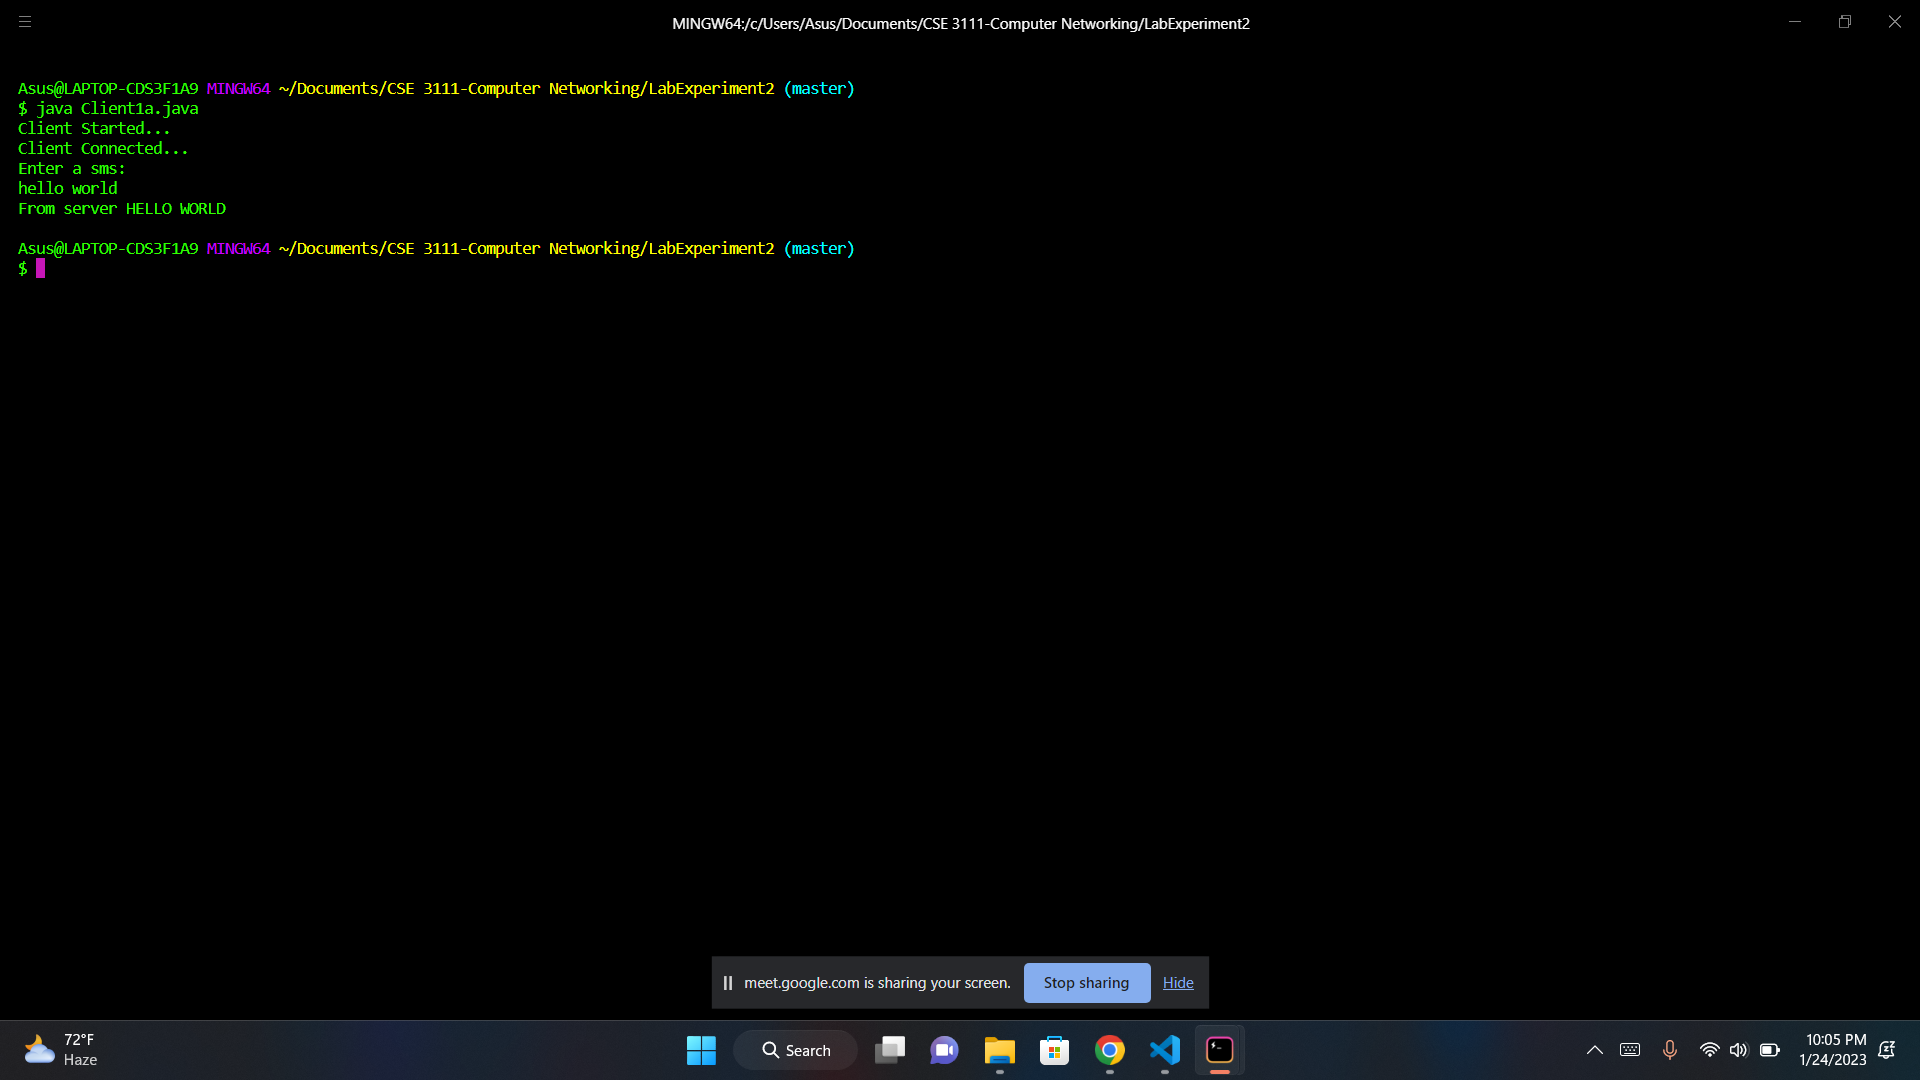
\includegraphics[width=\textwidth]{111.png}
\caption{Text sent from the client and capitalized text received}
\end{figure}

\begin{figure}[!h]
\centering
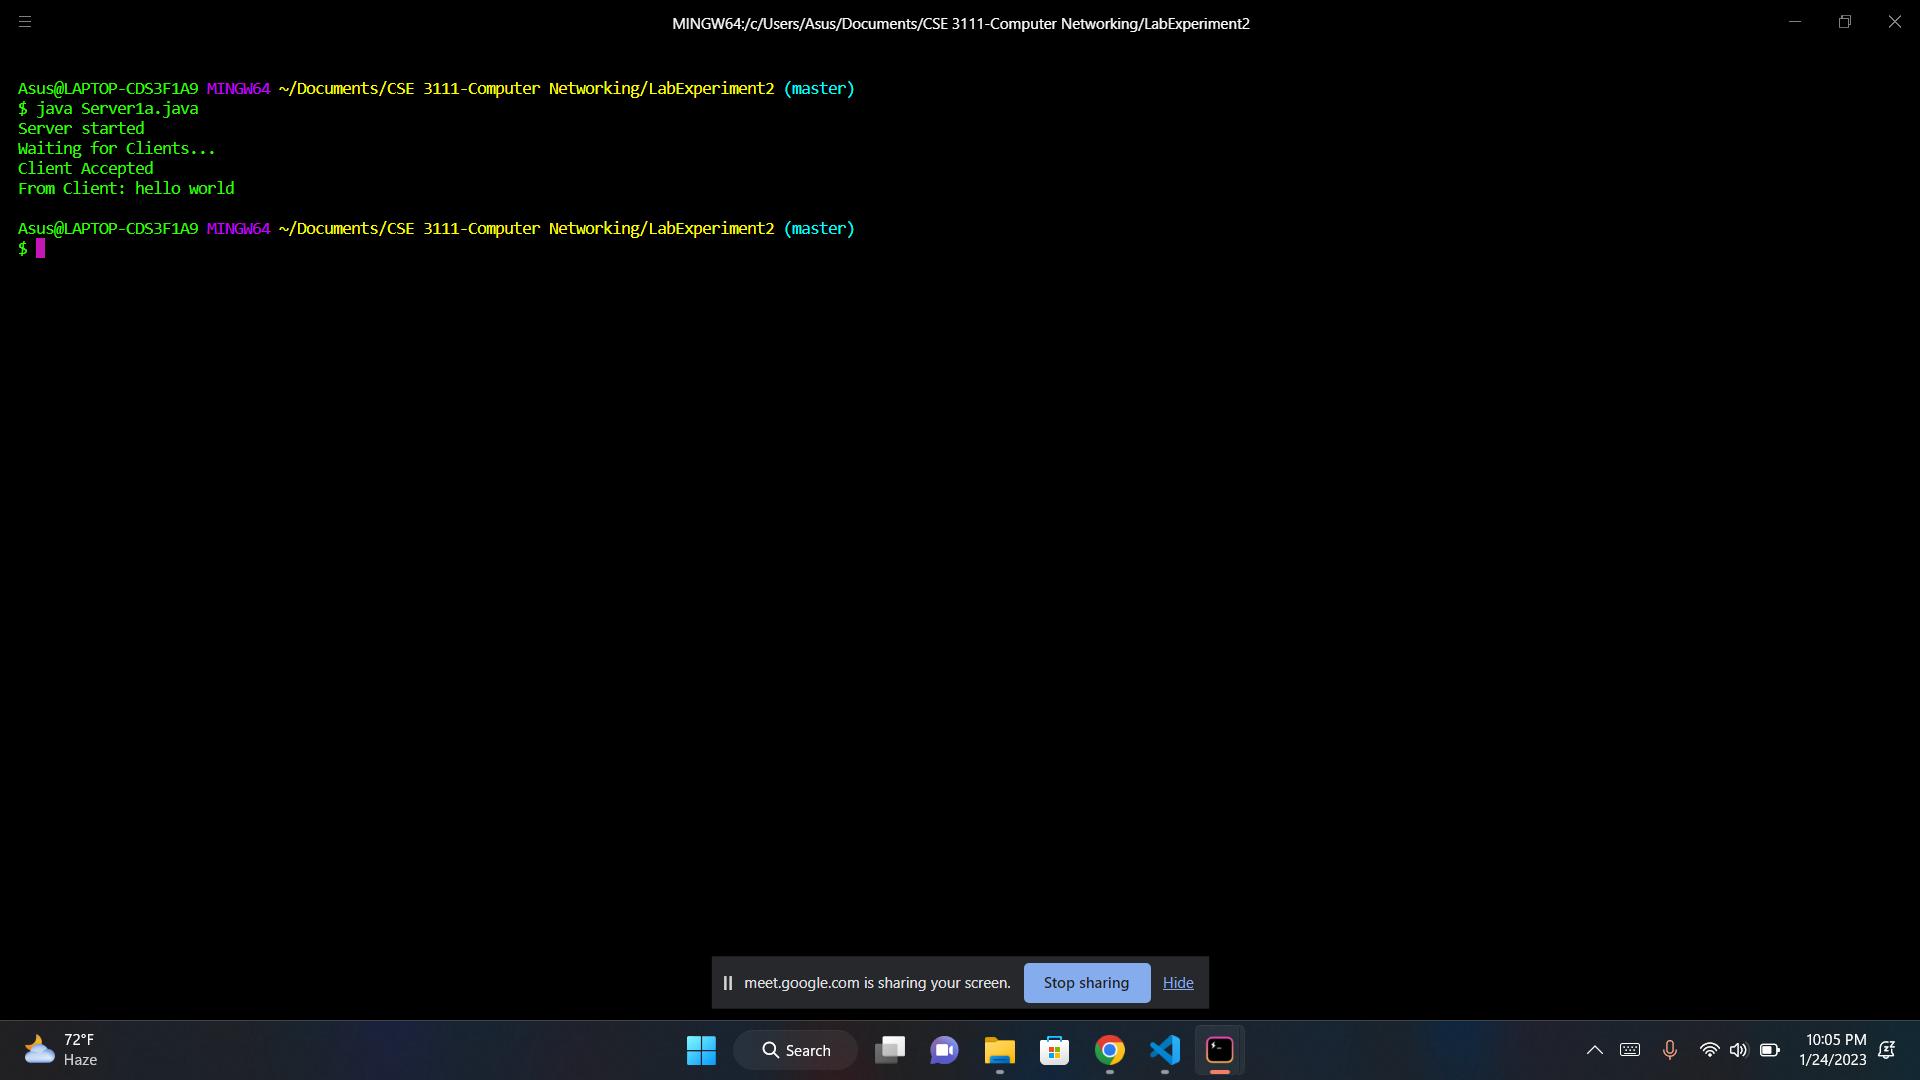
\includegraphics[width=\textwidth]{112.png}
\caption{Text received by the server and capitalized text sent}
\end{figure}

\newpage

\begin{figure}[!h]
\centering
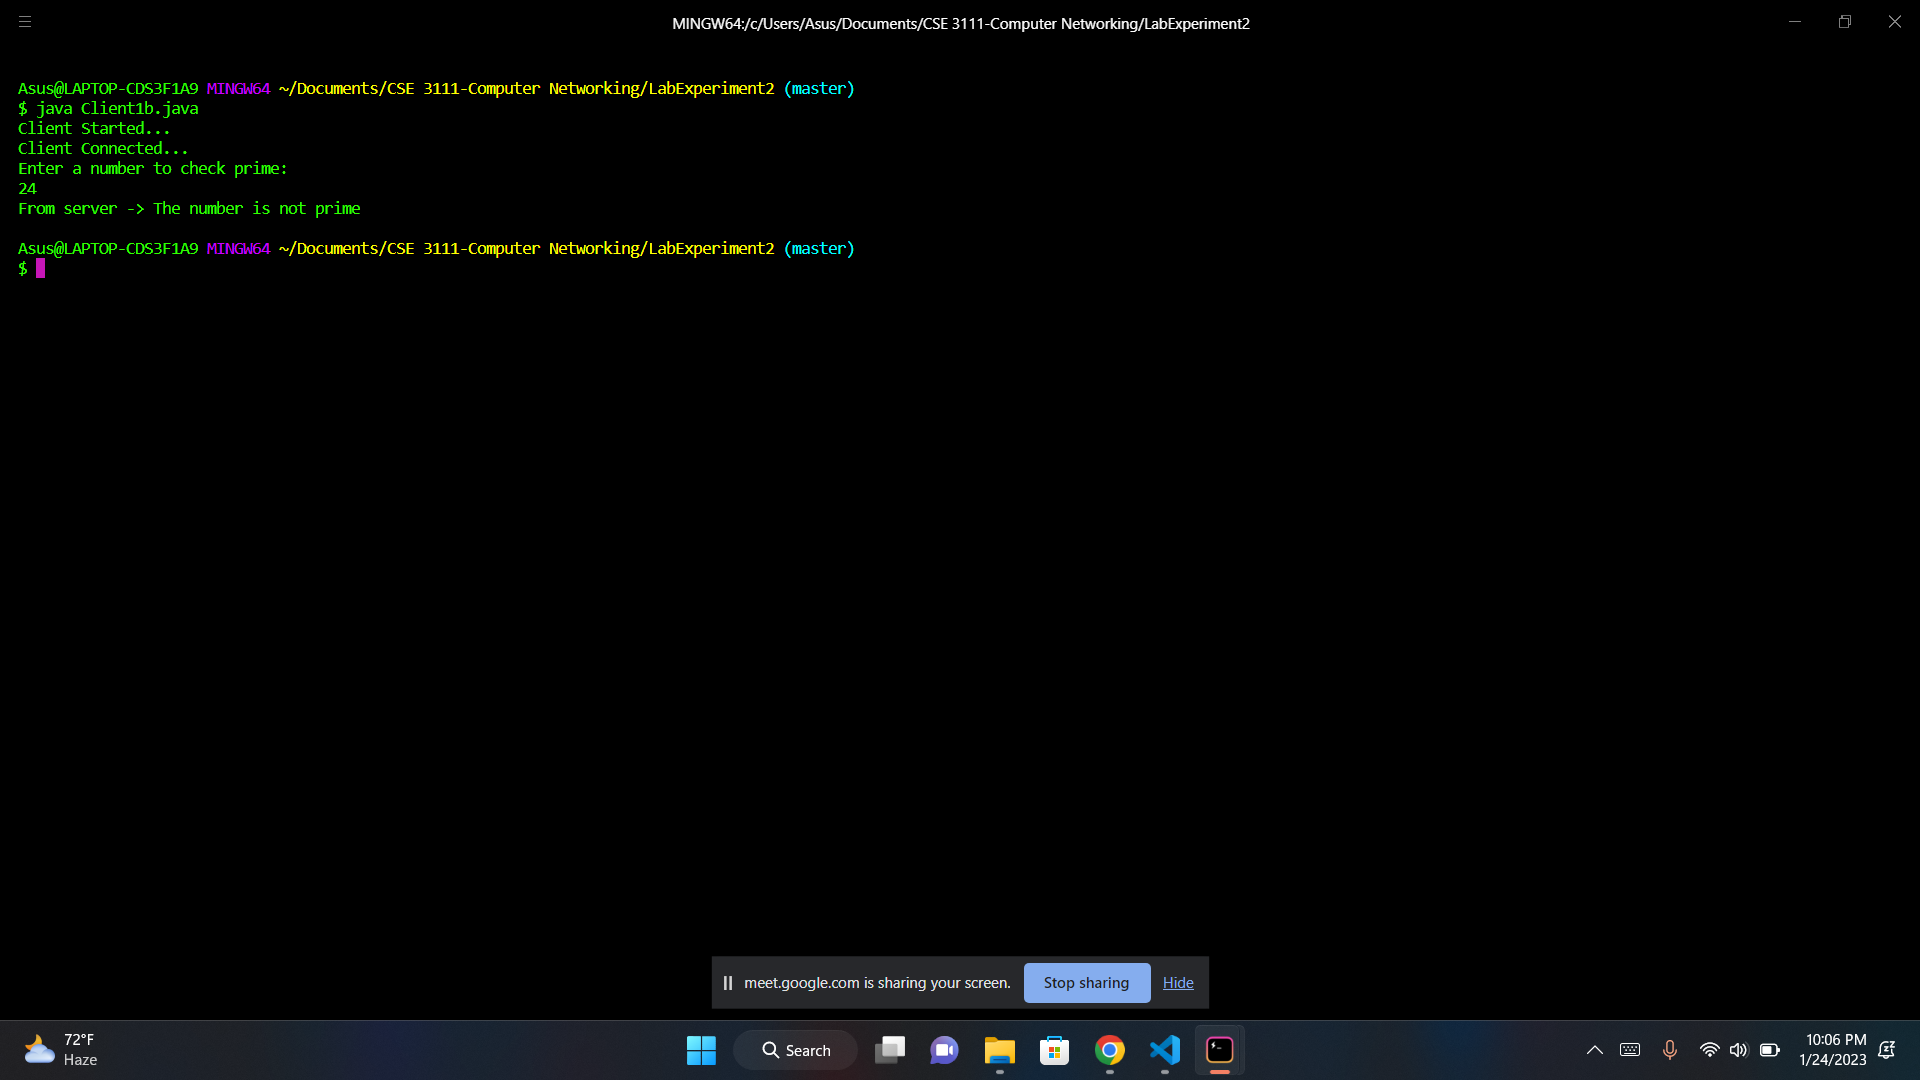
\includegraphics[width=\textwidth]{113.png}
\caption{Number sent from the client and primality check output shown (not prime)}
\end{figure}

\begin{figure}[!h]
\centering
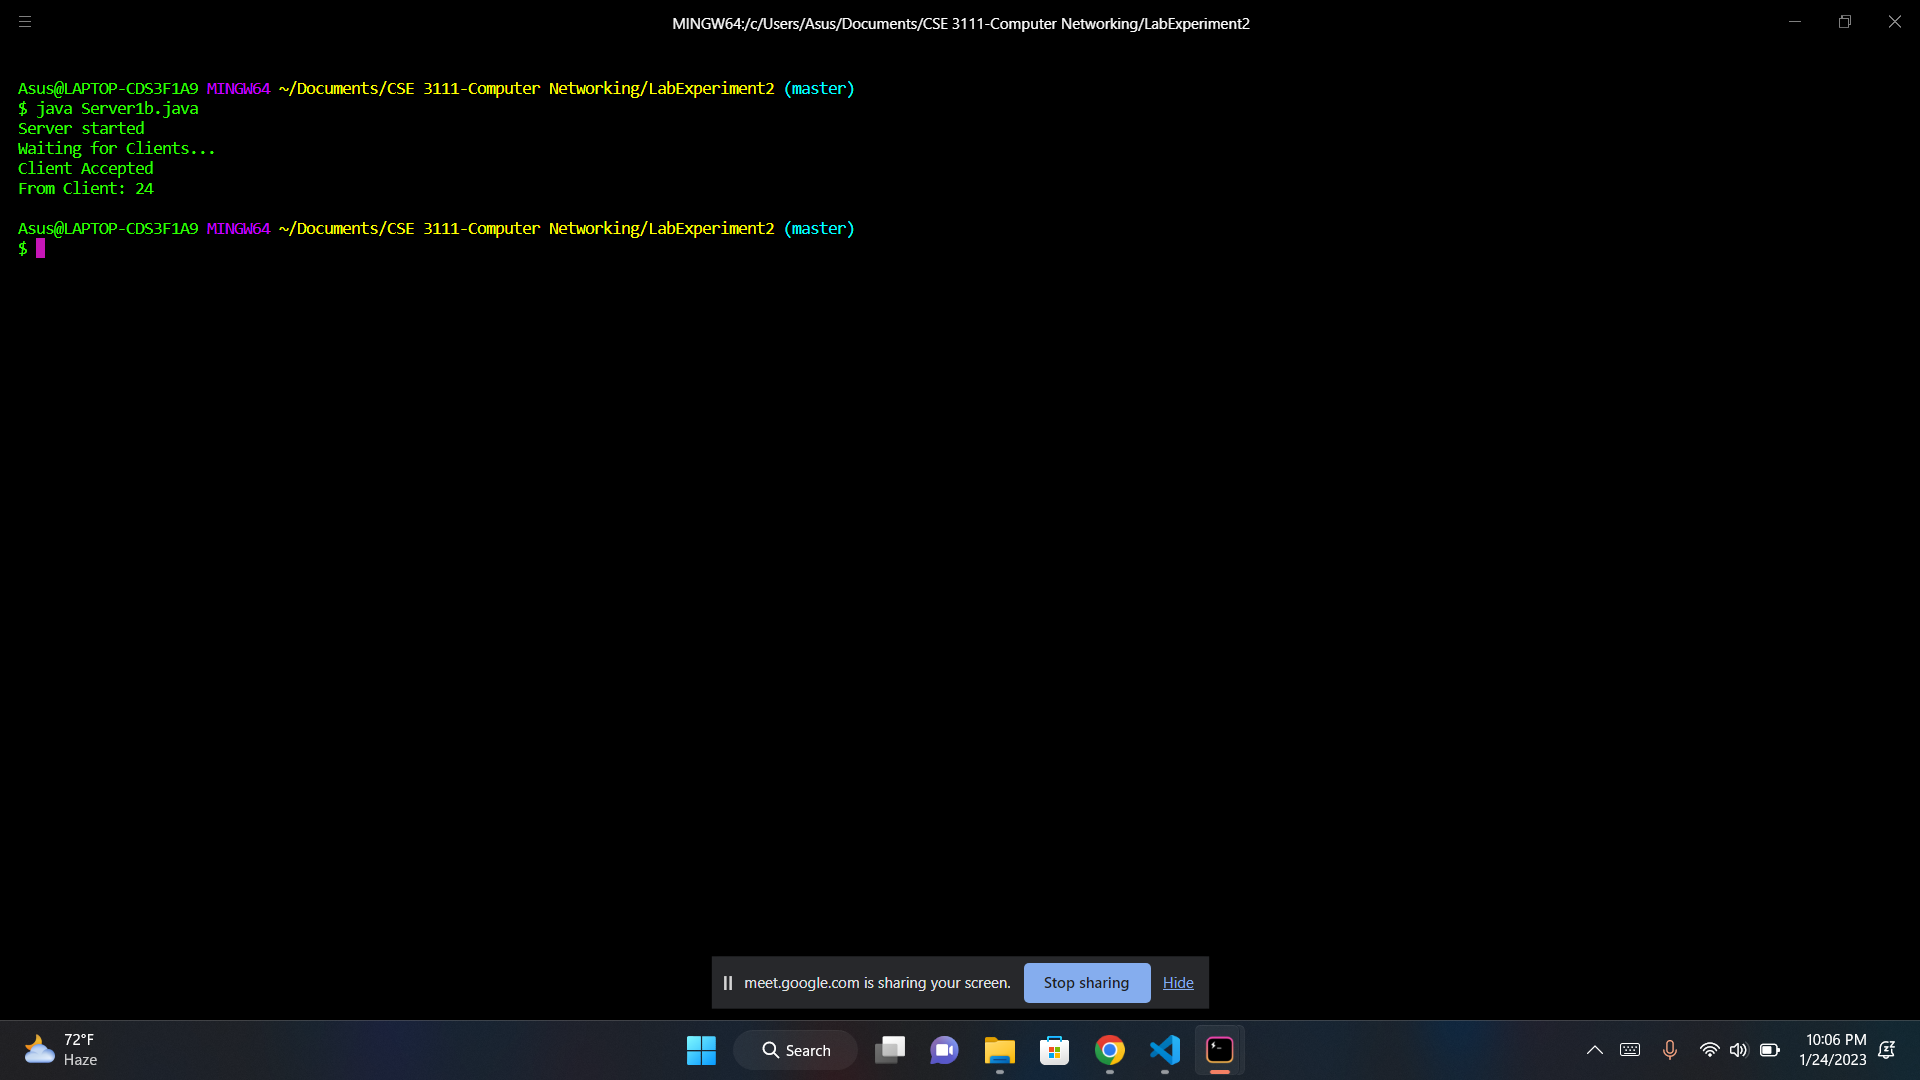
\includegraphics[width=\textwidth]{114.png}
\caption{Number received by the server and primality check is carried out}
\end{figure}

\newpage

\begin{figure}[!h]
\centering
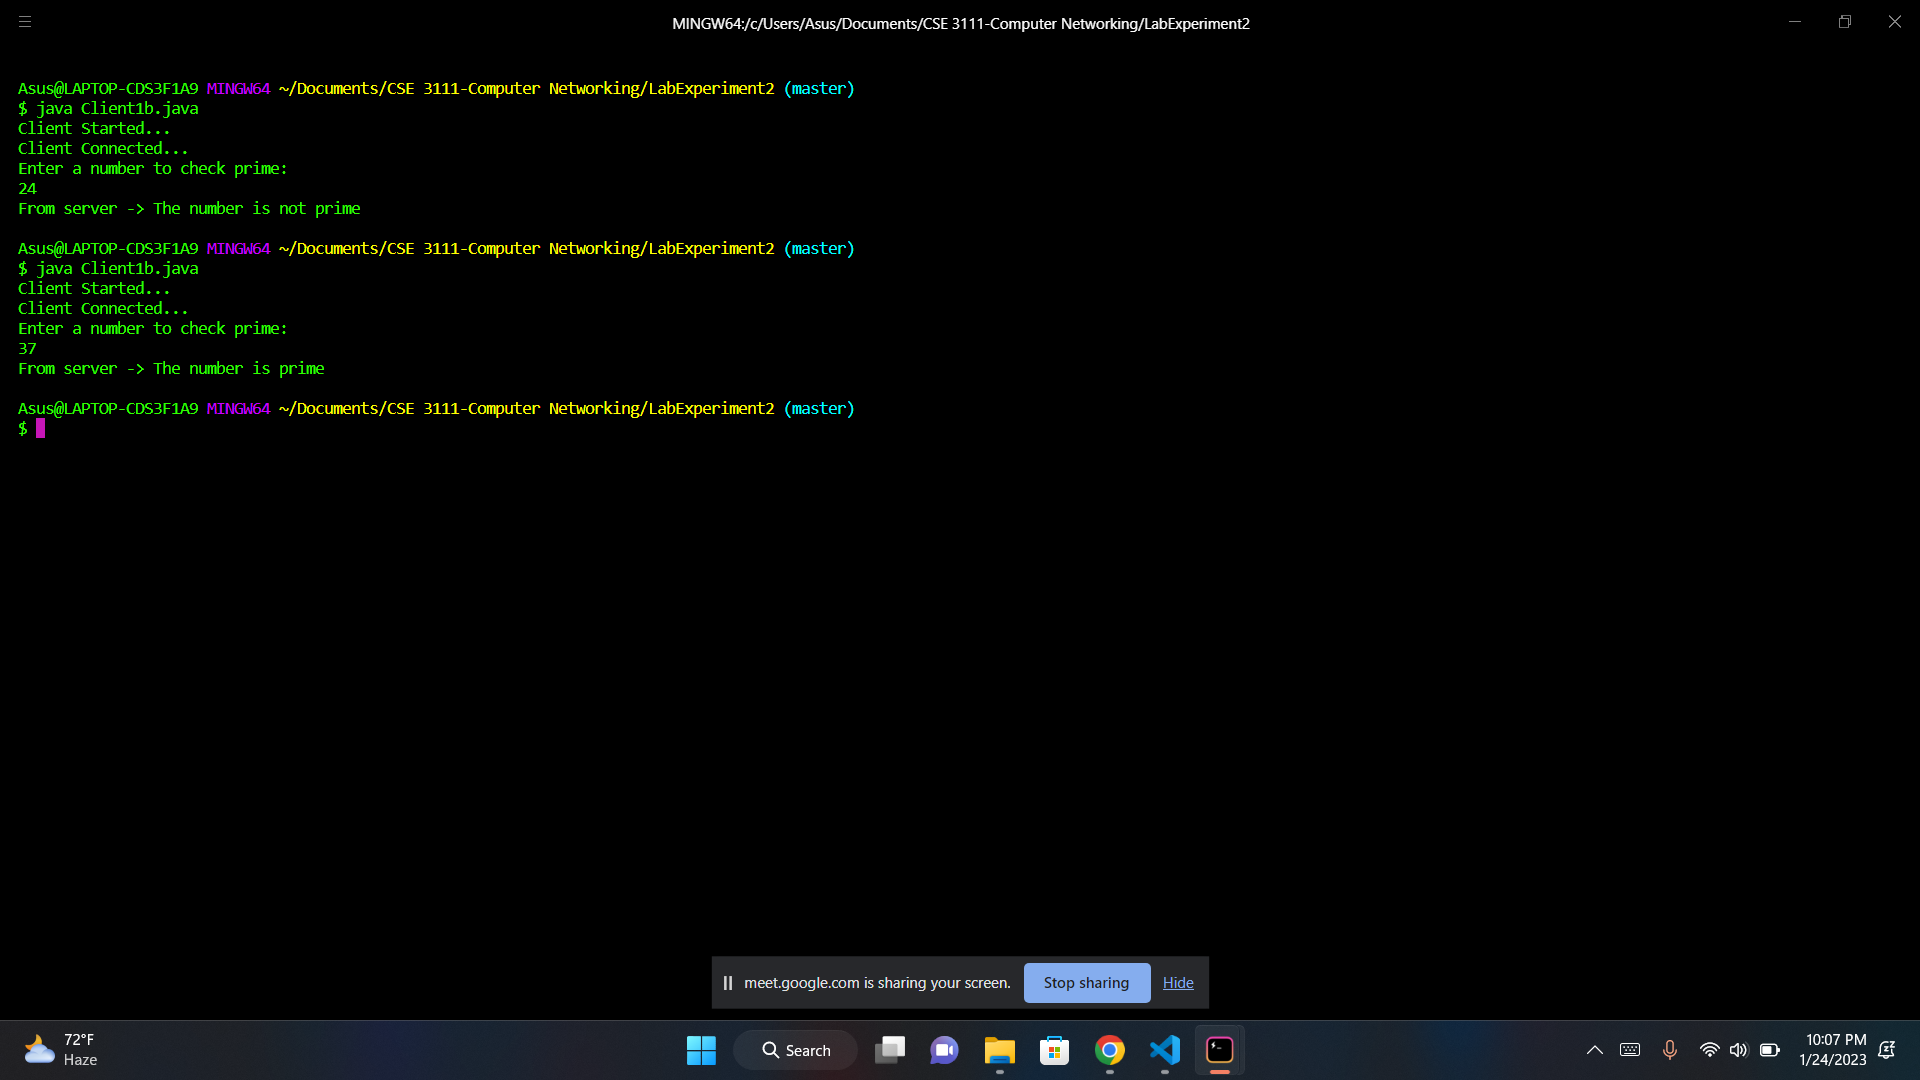
\includegraphics[width=\textwidth]{115.png}
\caption{Number sent from the client and primality check output shown (prime)}
\end{figure}

\begin{figure}[!h]
\centering
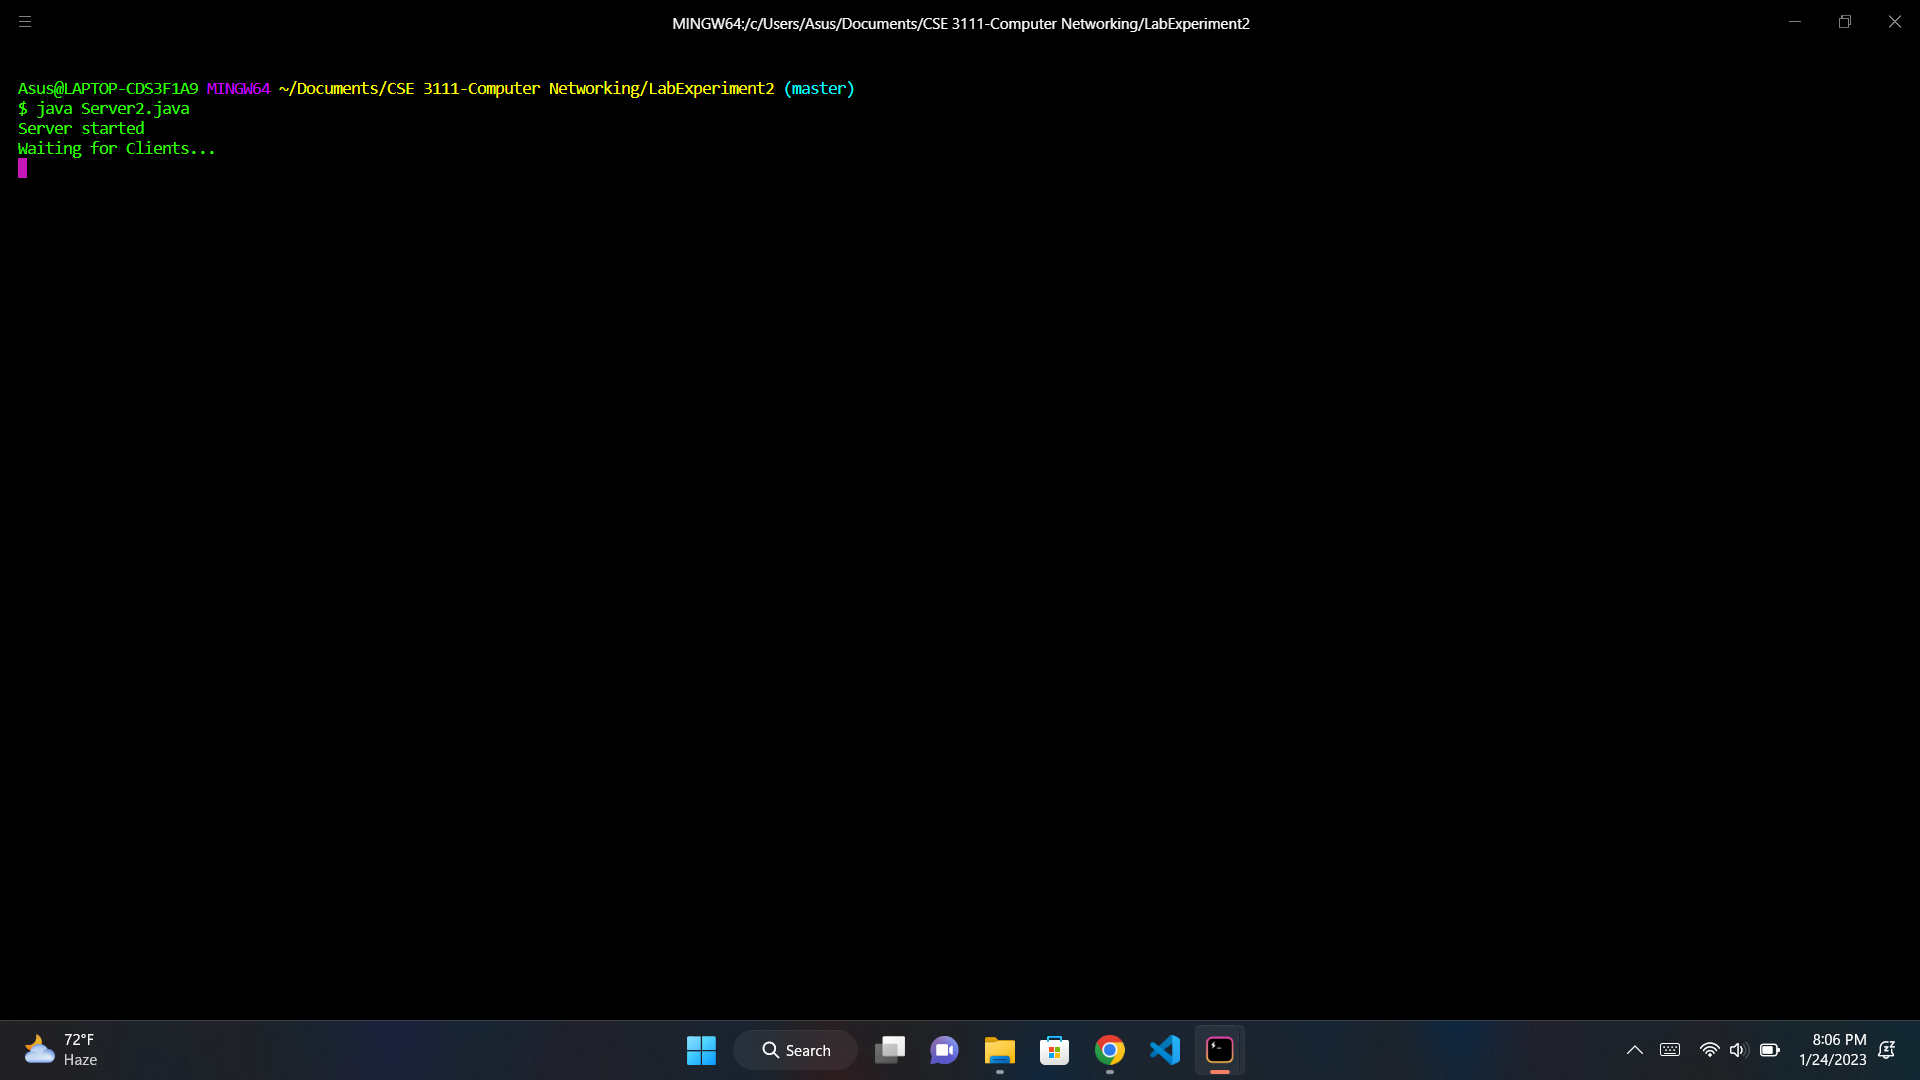
\includegraphics[width=\textwidth]{116.png}
\caption{ATM server started}
\end{figure}


\newpage


\begin{figure}[!h]
\centering
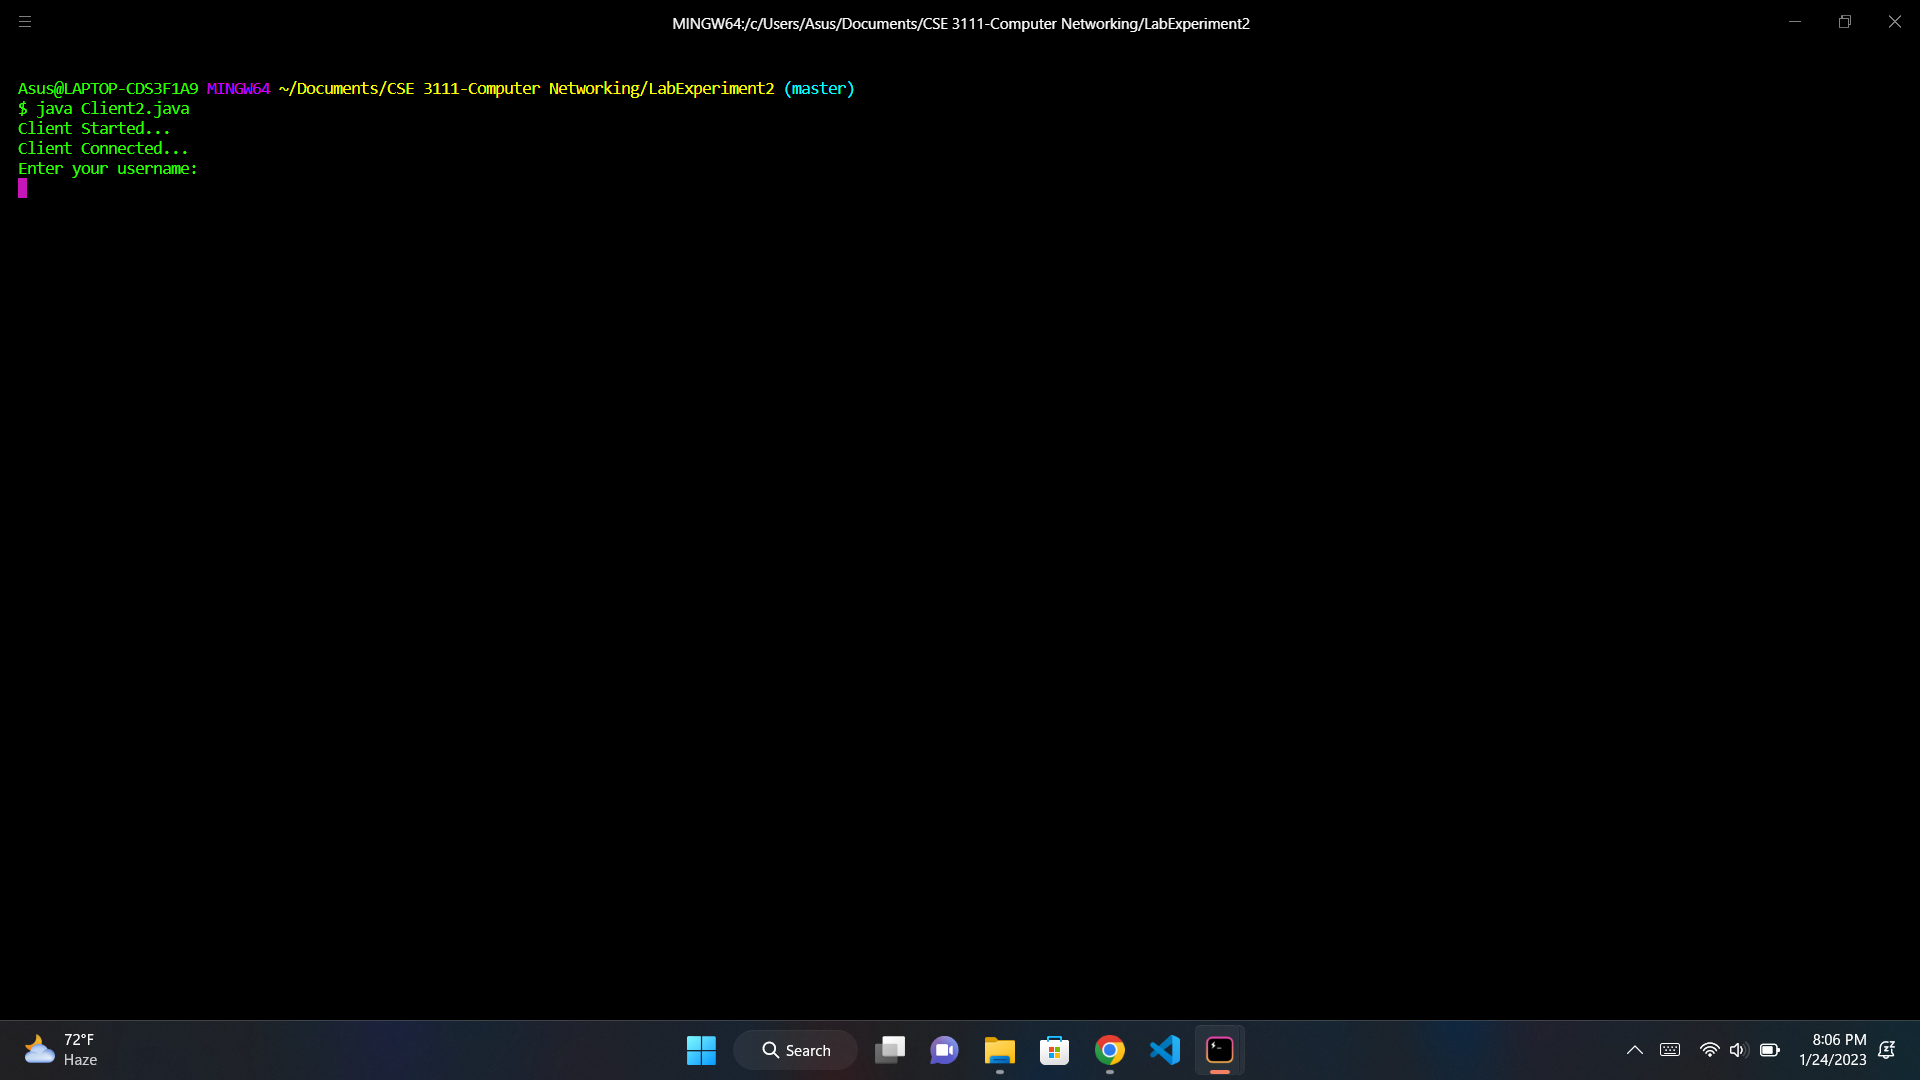
\includegraphics[width=\textwidth]{117.png}
\caption{ATM client started}
\end{figure}

\begin{figure}[!h]
\centering
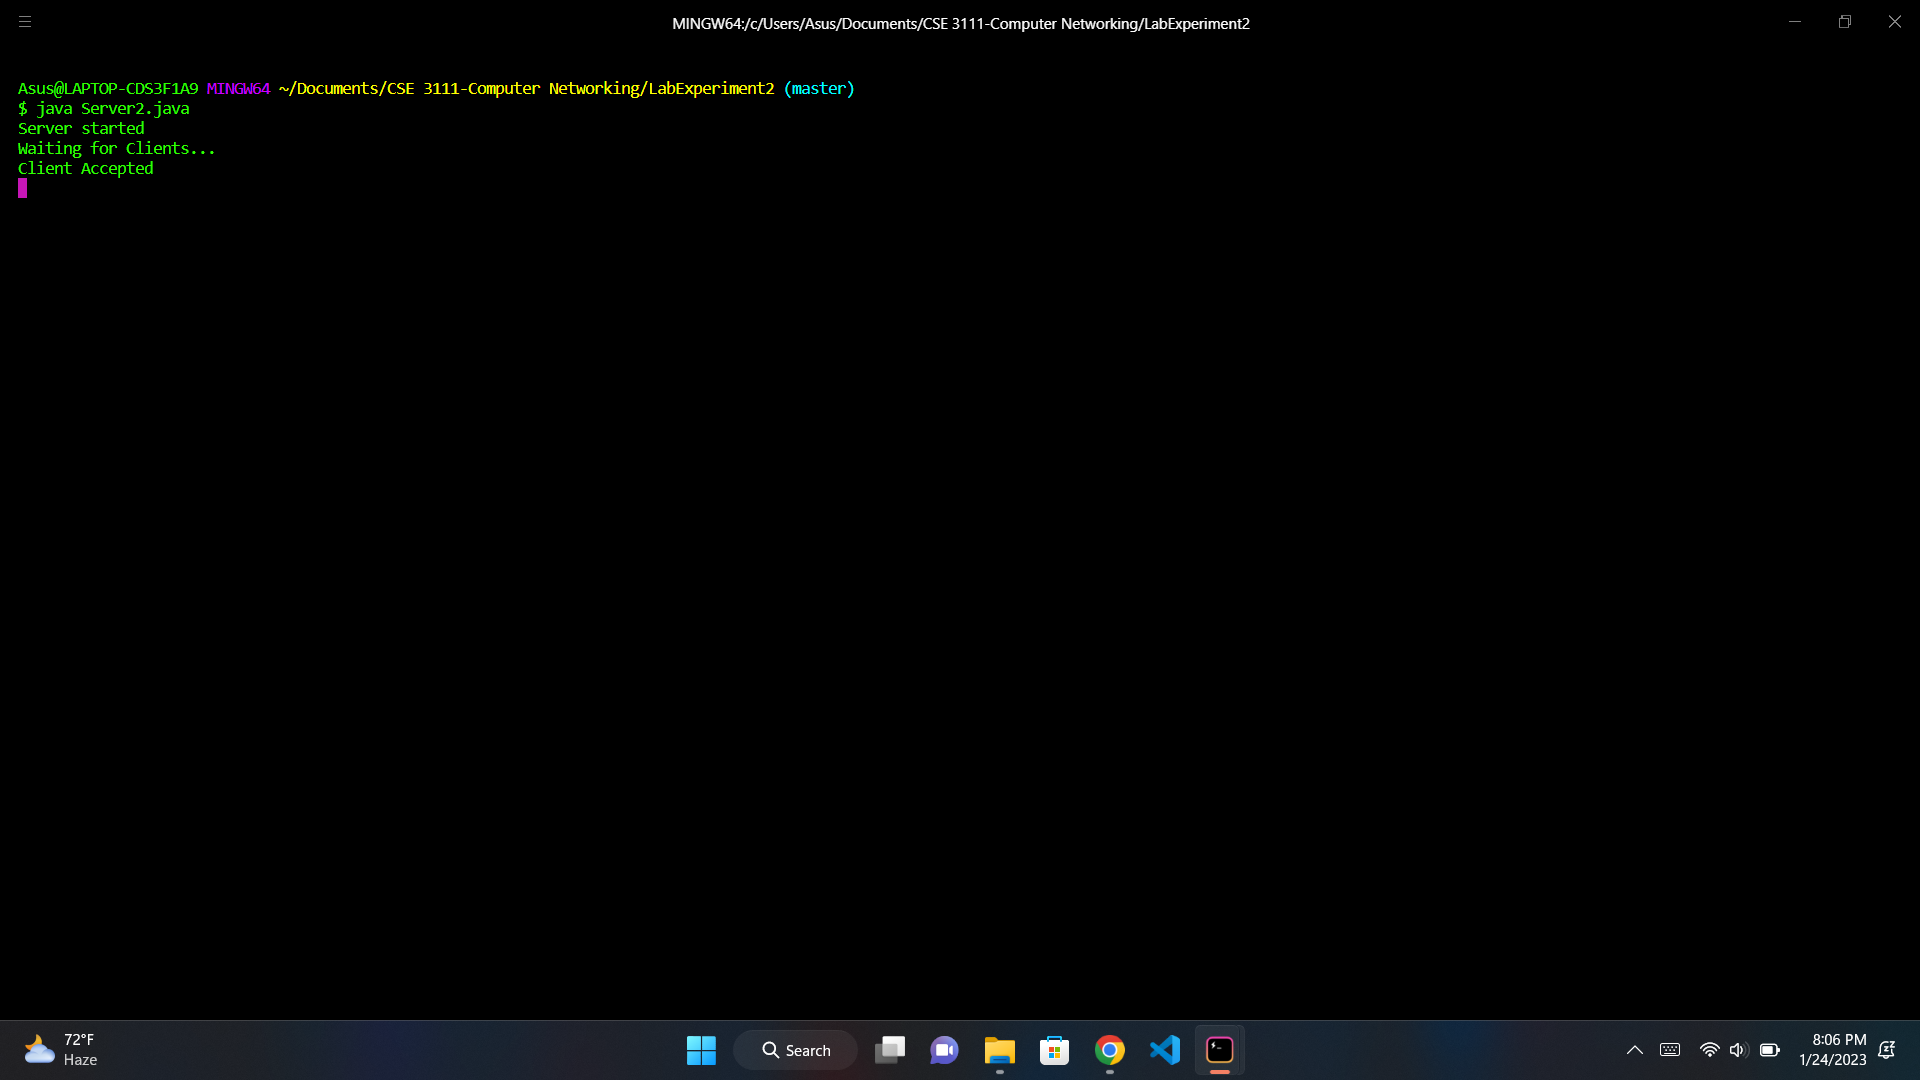
\includegraphics[width=\textwidth]{118.png}
\caption{Client accepted by server}
\end{figure}

\newpage


\begin{figure}[!h]
\centering
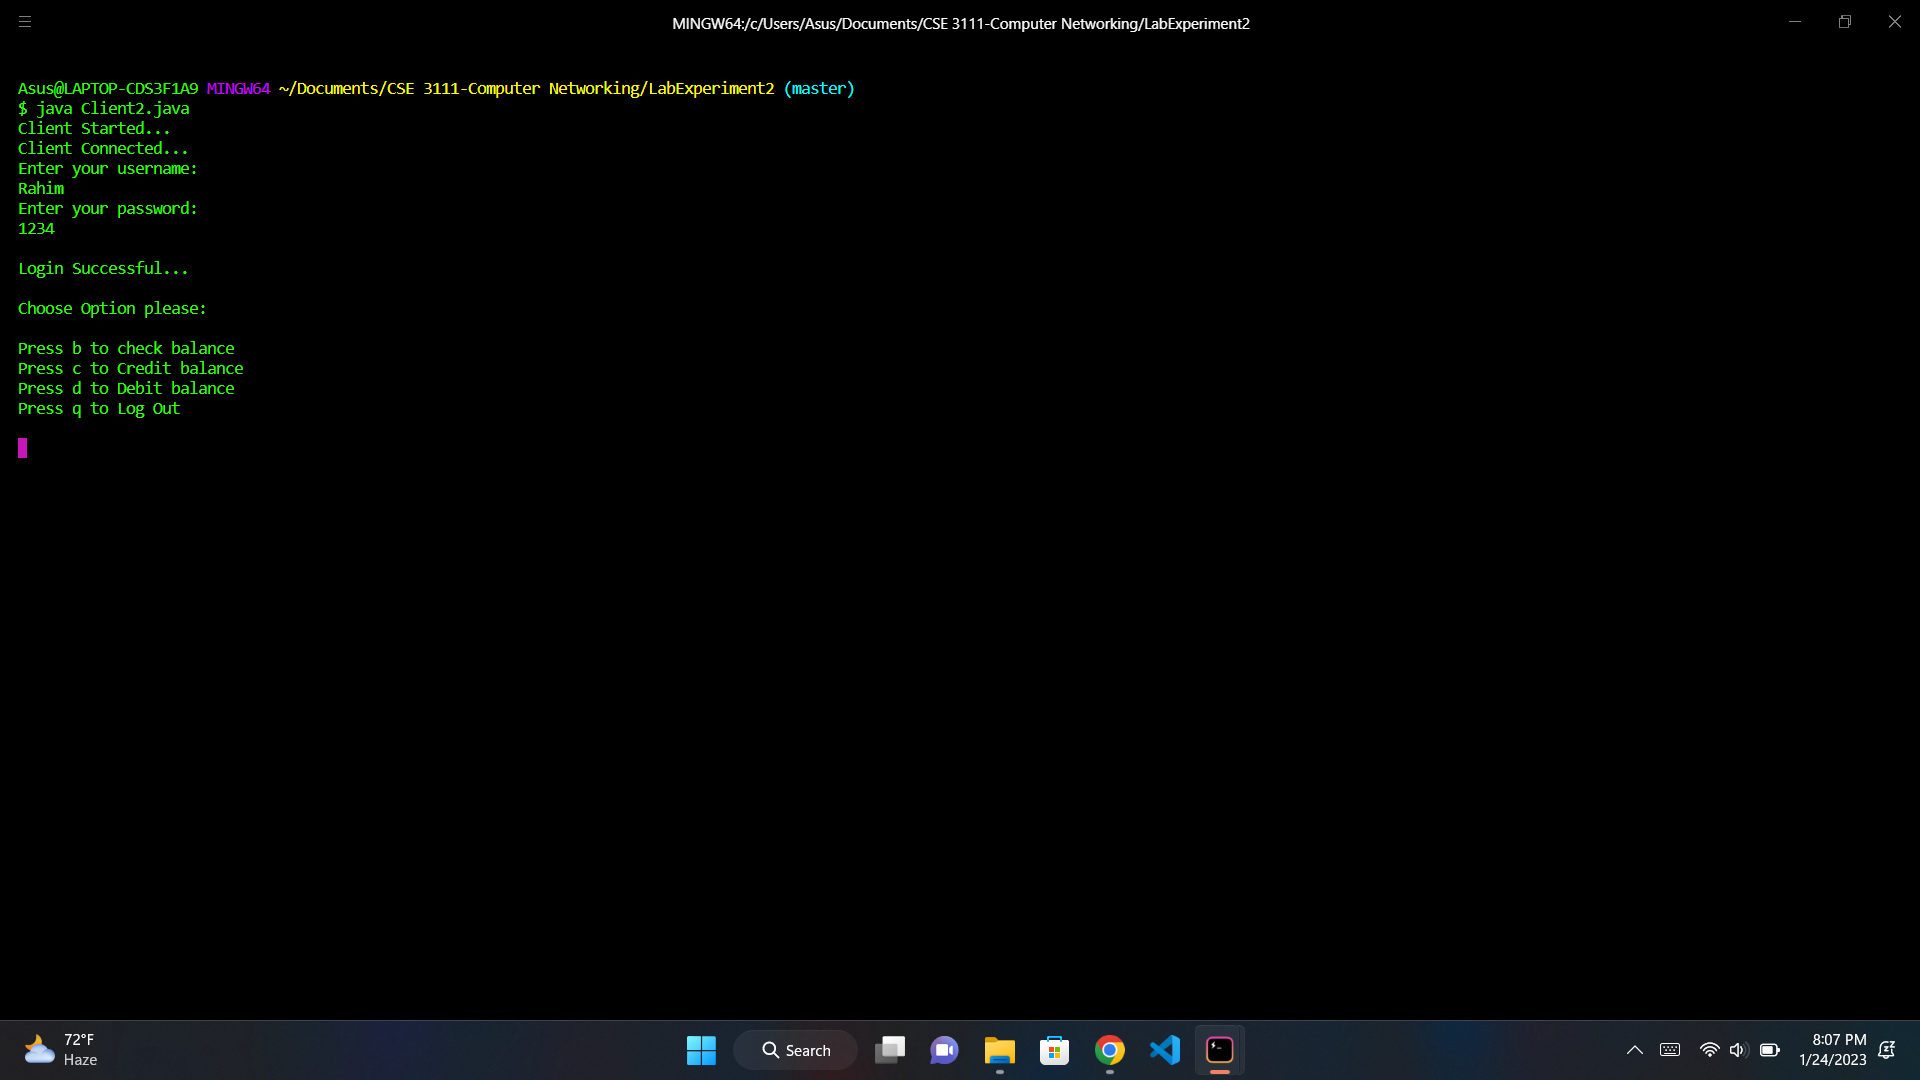
\includegraphics[width=\textwidth]{119.png}
\caption{ATM user login and user menu}
\end{figure}

\begin{figure}[!h]
\centering
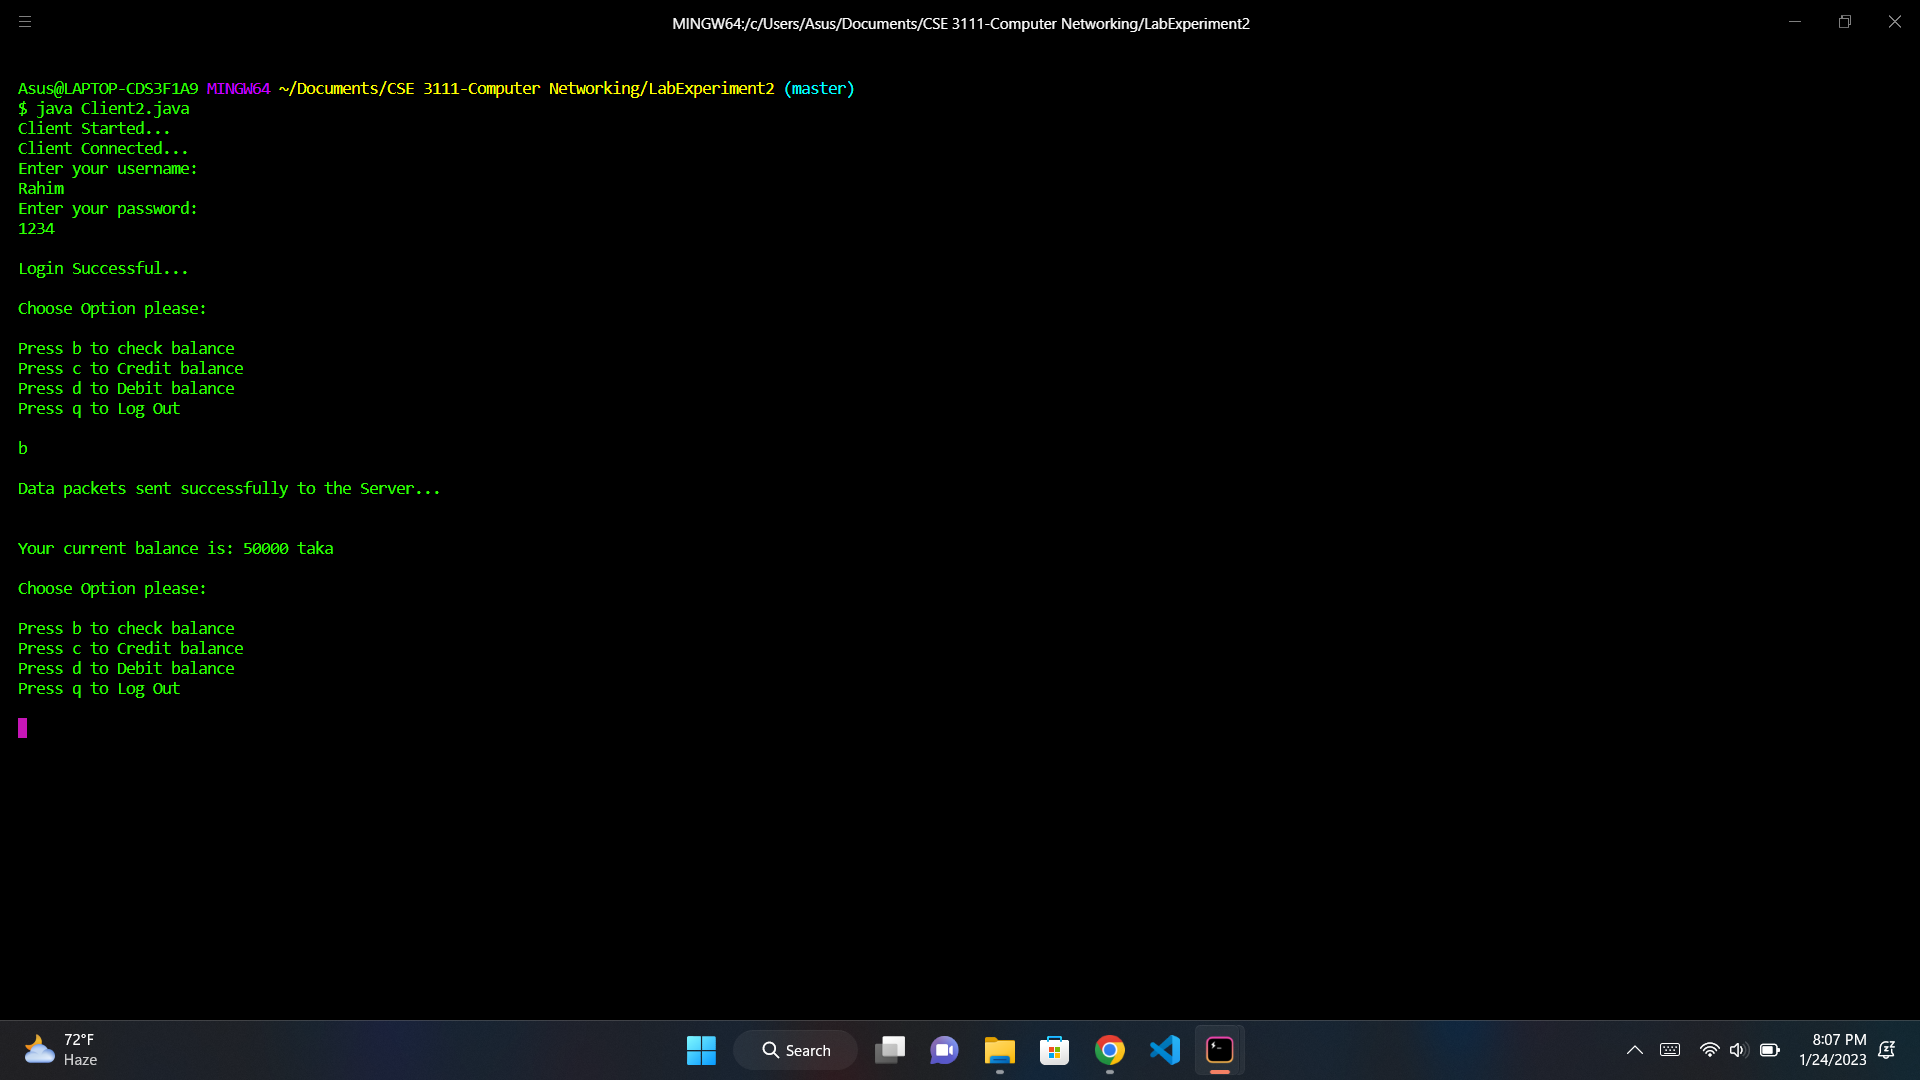
\includegraphics[width=\textwidth]{120.png}
\caption{User checking balance. Data packets sent without any error.}
\end{figure}

\newpage

\begin{figure}[!h]
\centering
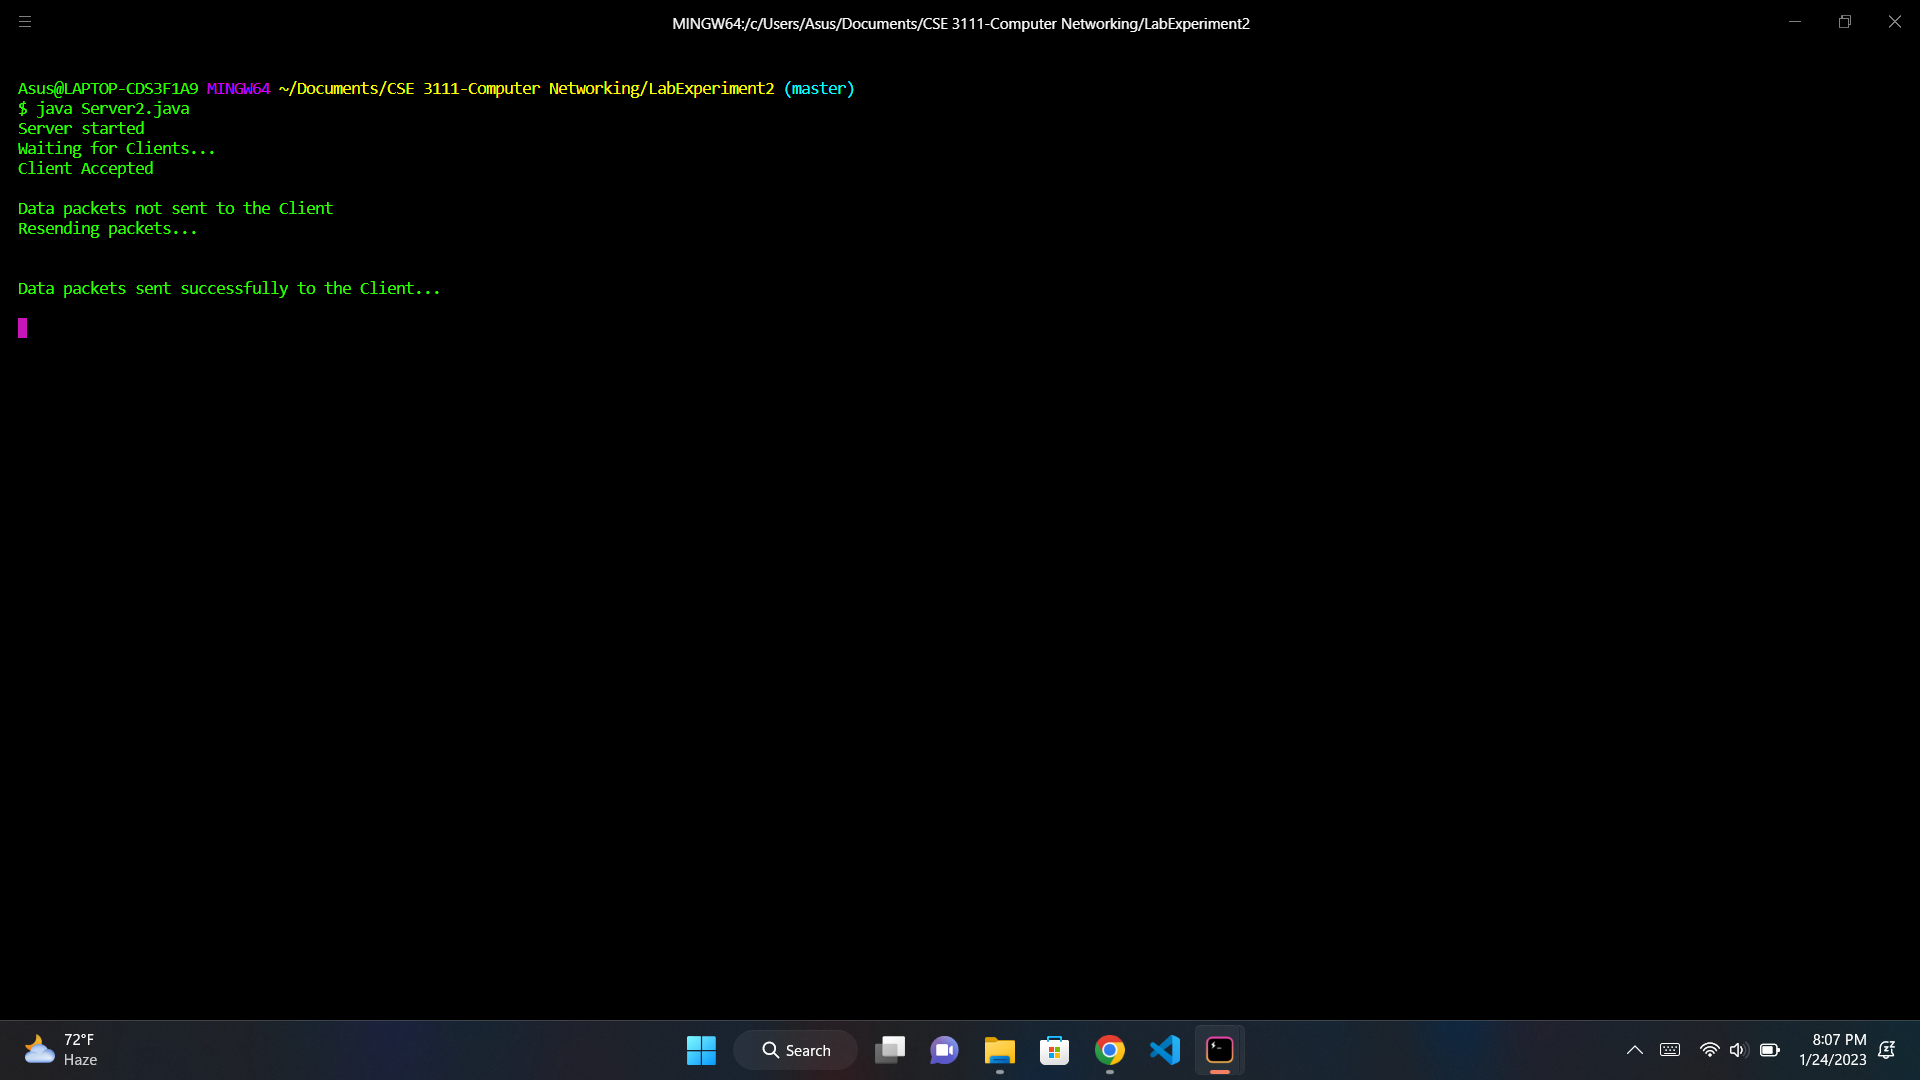
\includegraphics[width=\textwidth]{121.png}
\caption{ Data packets sent to client from server after 1 error.}
\end{figure}



\begin{figure}[!h]
\centering
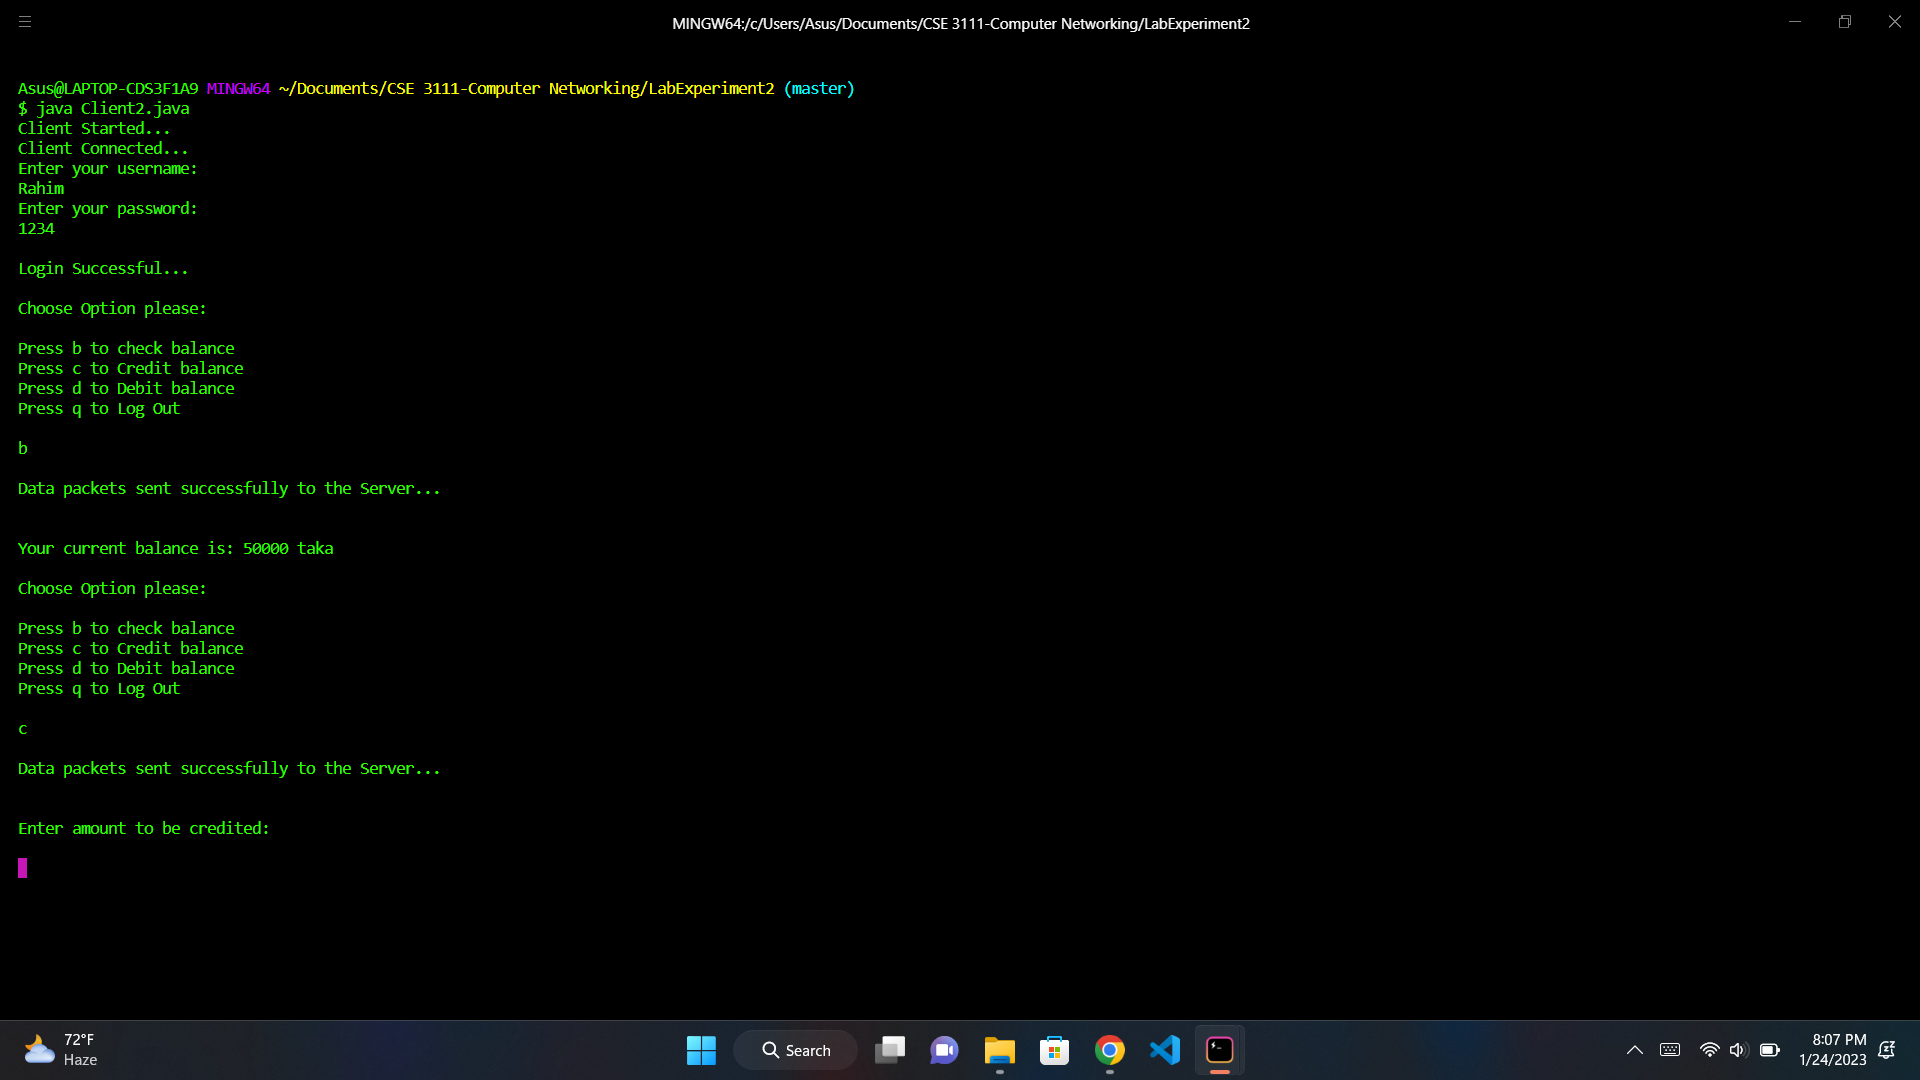
\includegraphics[width=\textwidth]{122.png}
\caption{ User chooses to credit balance}
\end{figure}


\newpage

\begin{figure}[!h]
\centering
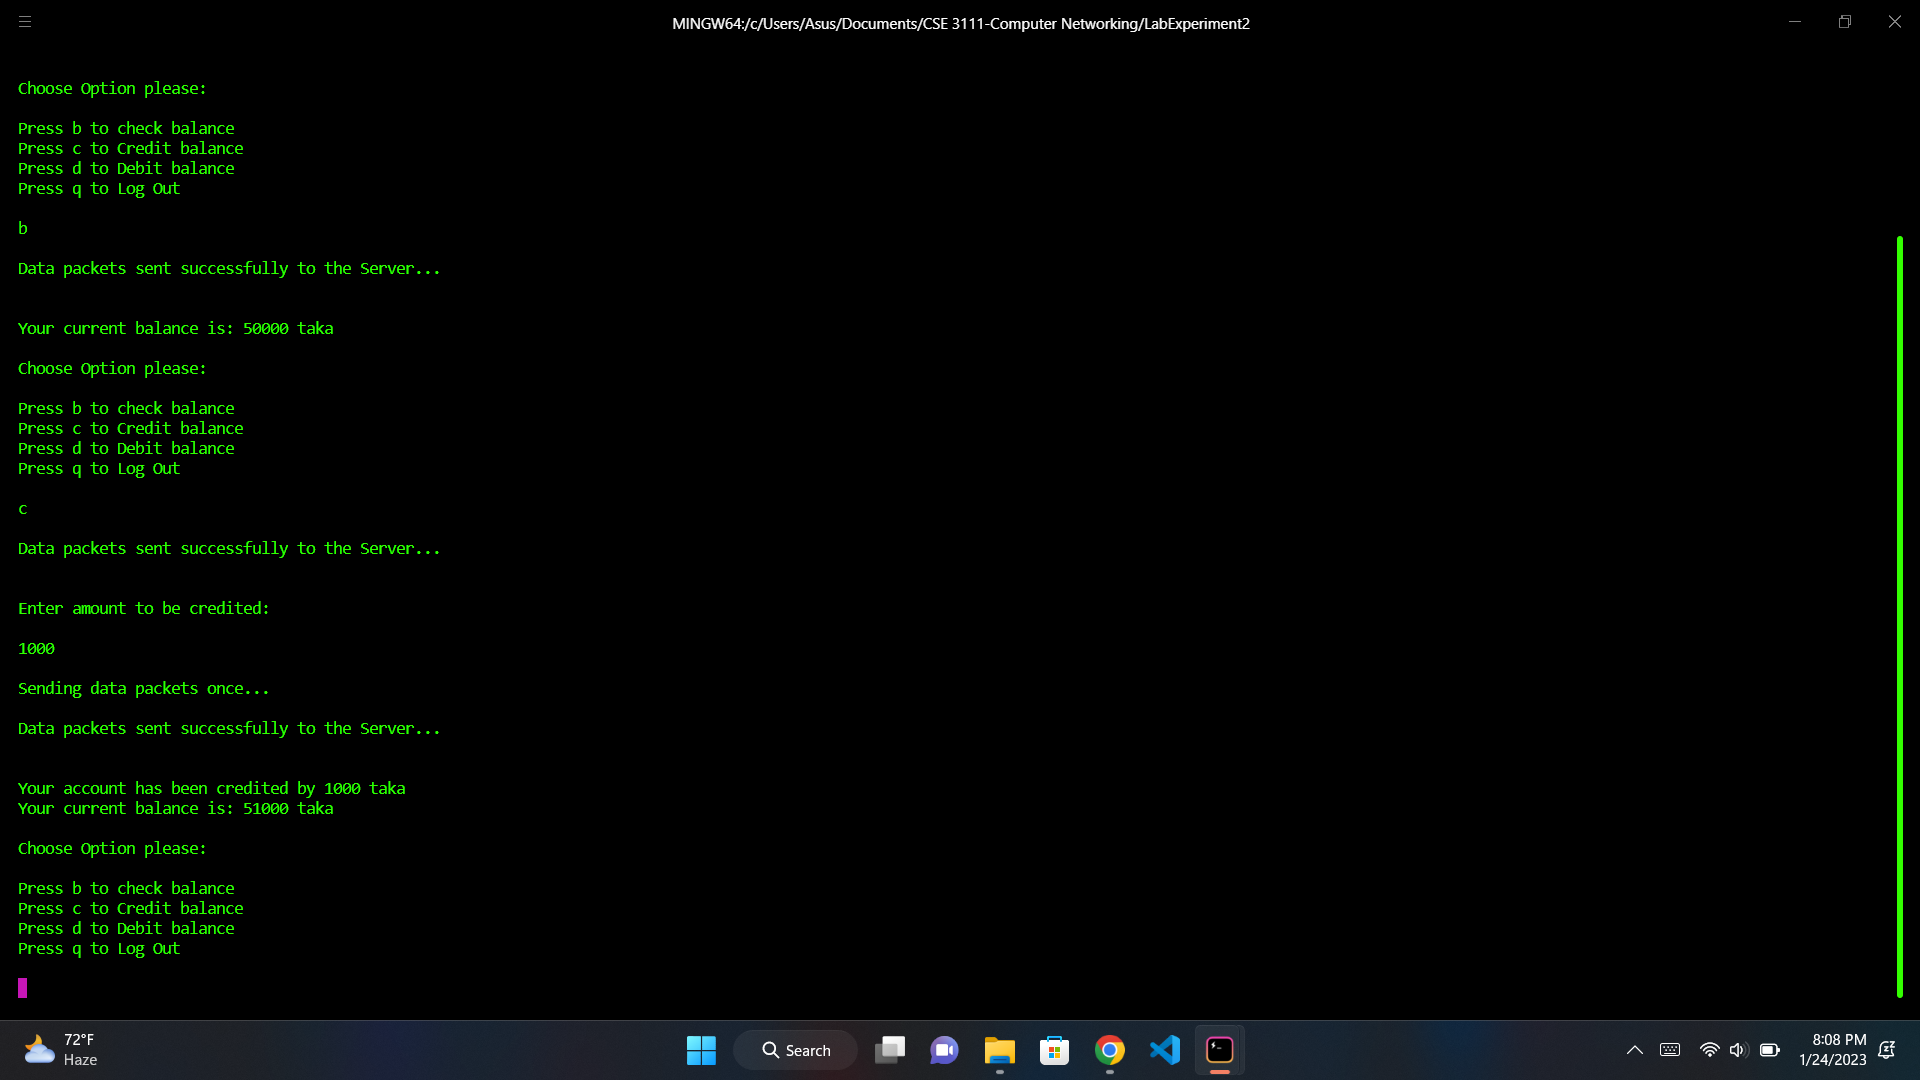
\includegraphics[width=\textwidth]{123.png}
\caption{ User gives the amount to be credited. Data is sent once}
\end{figure}


\begin{figure}[!h]
\centering
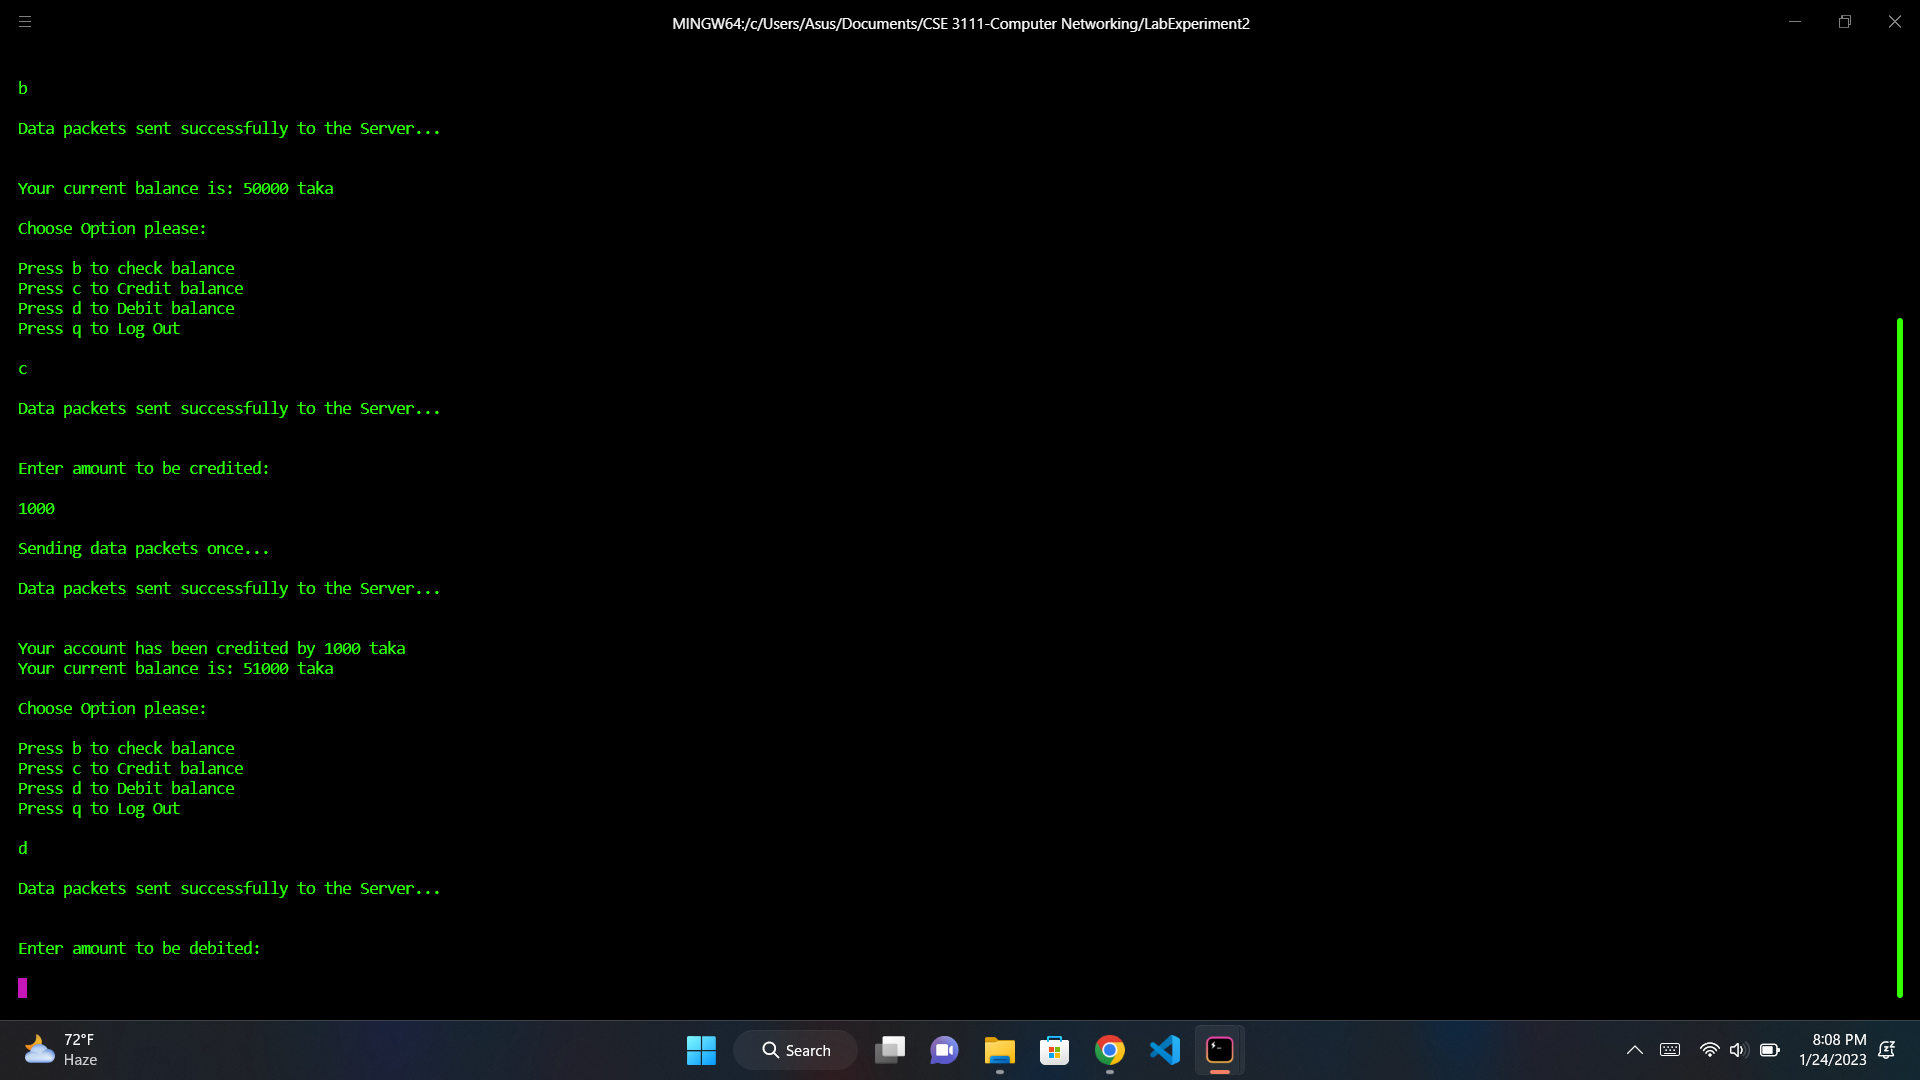
\includegraphics[width=\textwidth]{124.png}
\caption{User chooses to debit balance}
\end{figure}

\newpage

\begin{figure}[!h]
\centering
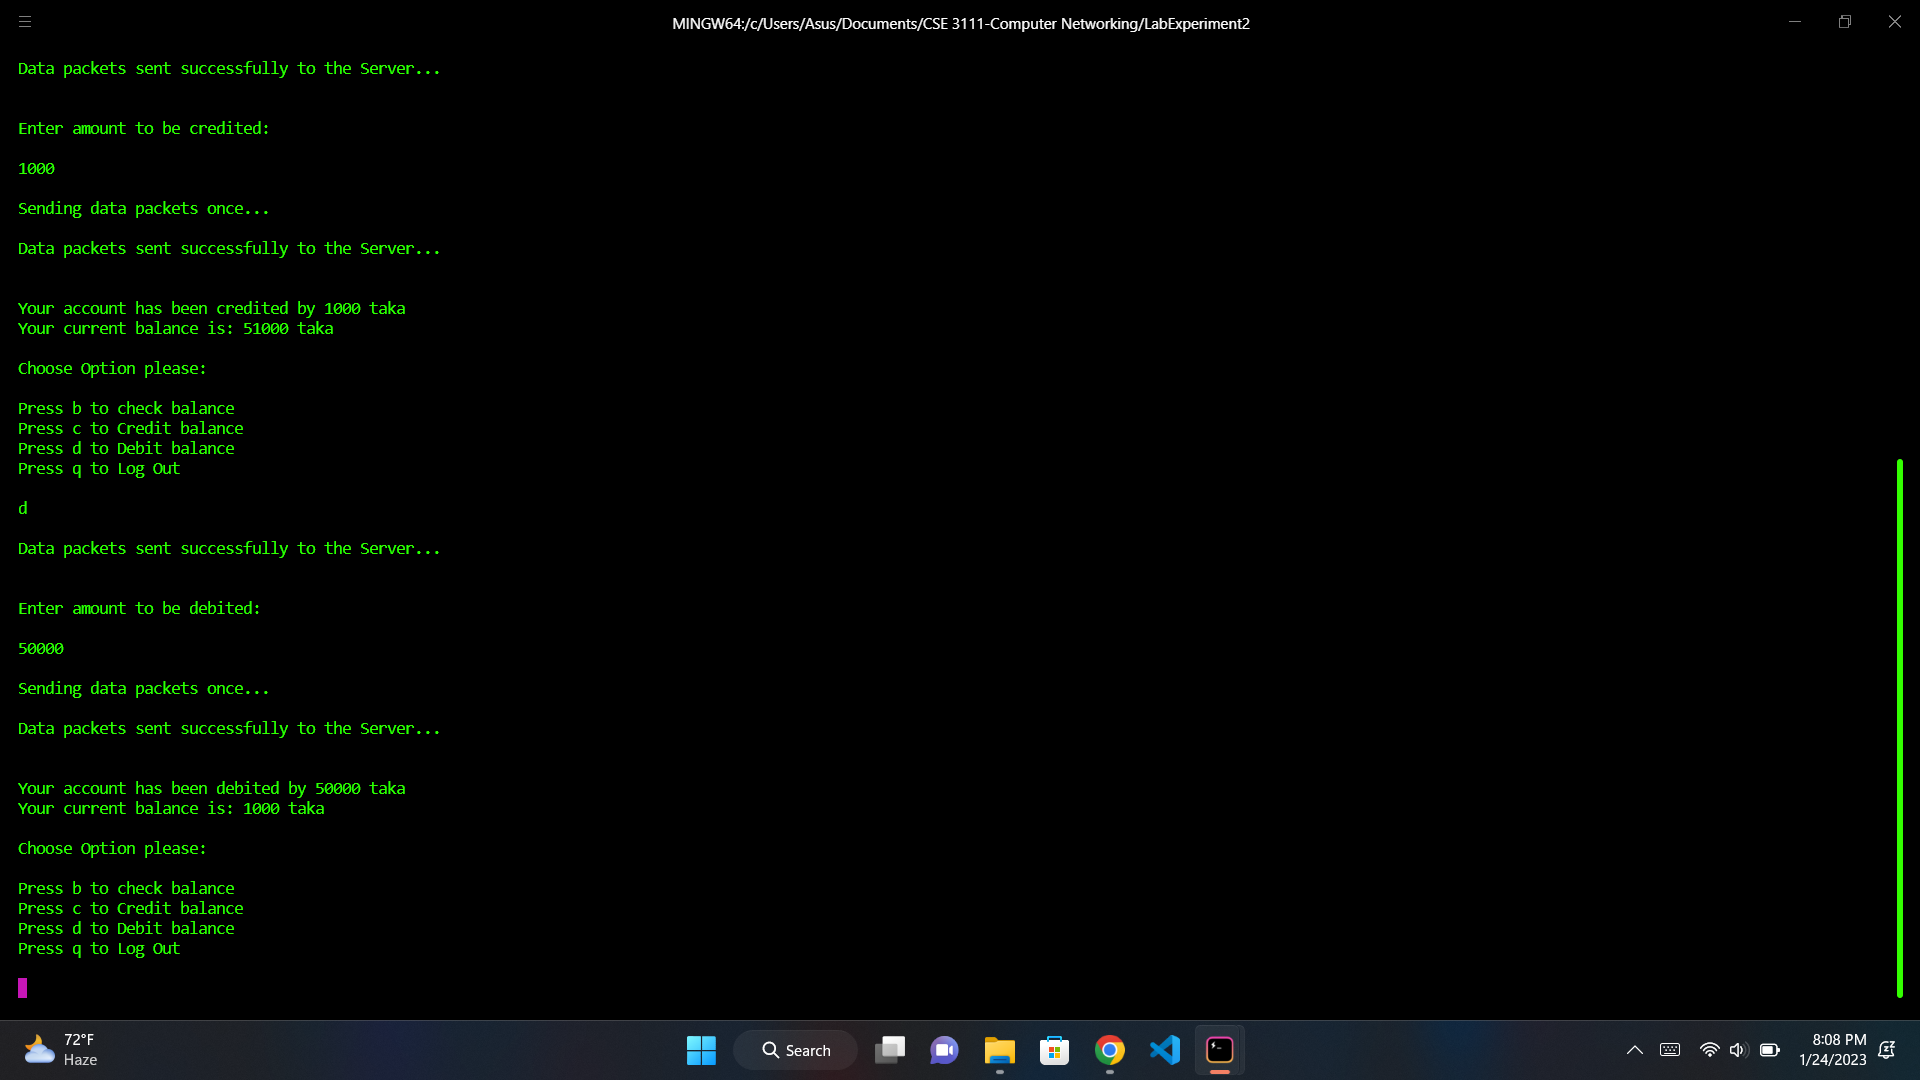
\includegraphics[width=\textwidth]{125.png}
\caption{User gives the amount to be debited. Data is sent once.}
\end{figure}



\begin{figure}[!h]
\centering
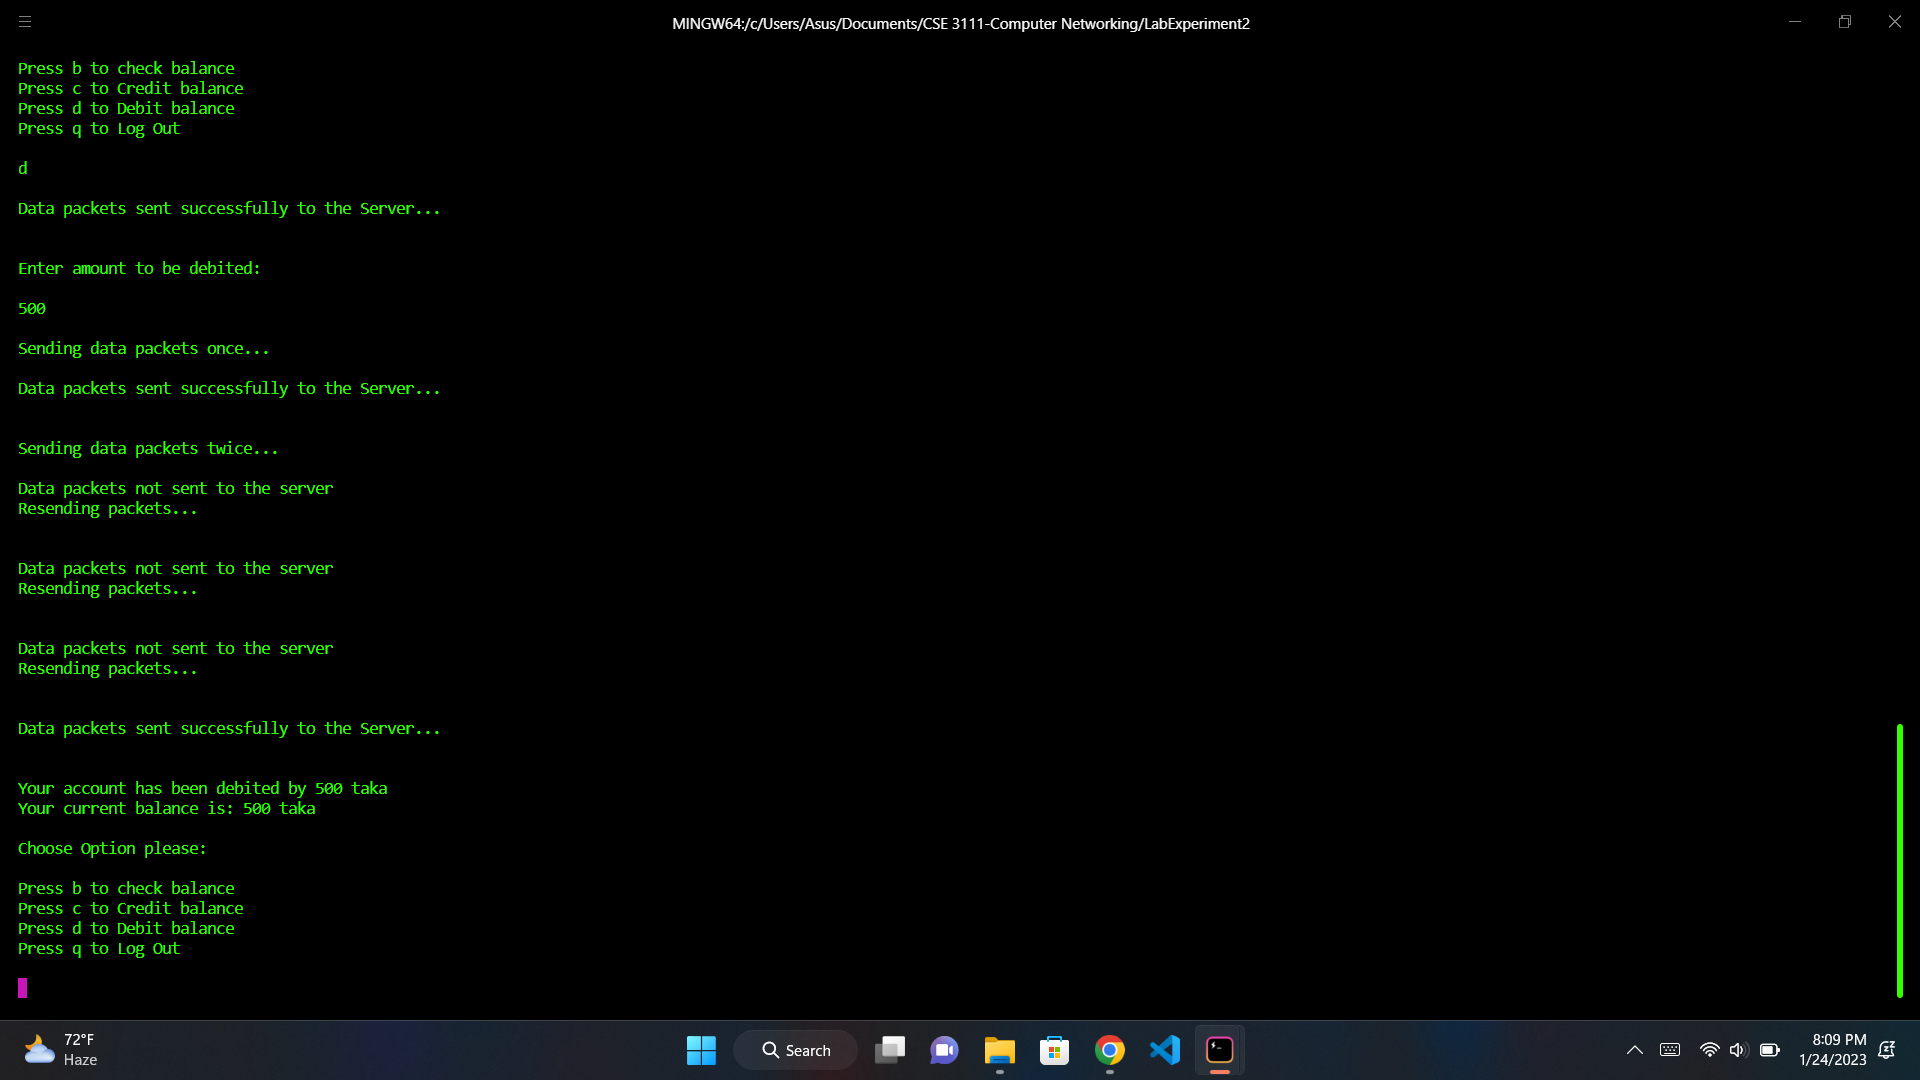
\includegraphics[width=\textwidth]{126.png}
\caption{User chooses to debit the balance. This time the operation is sent twice, but the debit operation is carried out only once.}
\end{figure}

\newpage

\begin{figure}[!h]
\centering
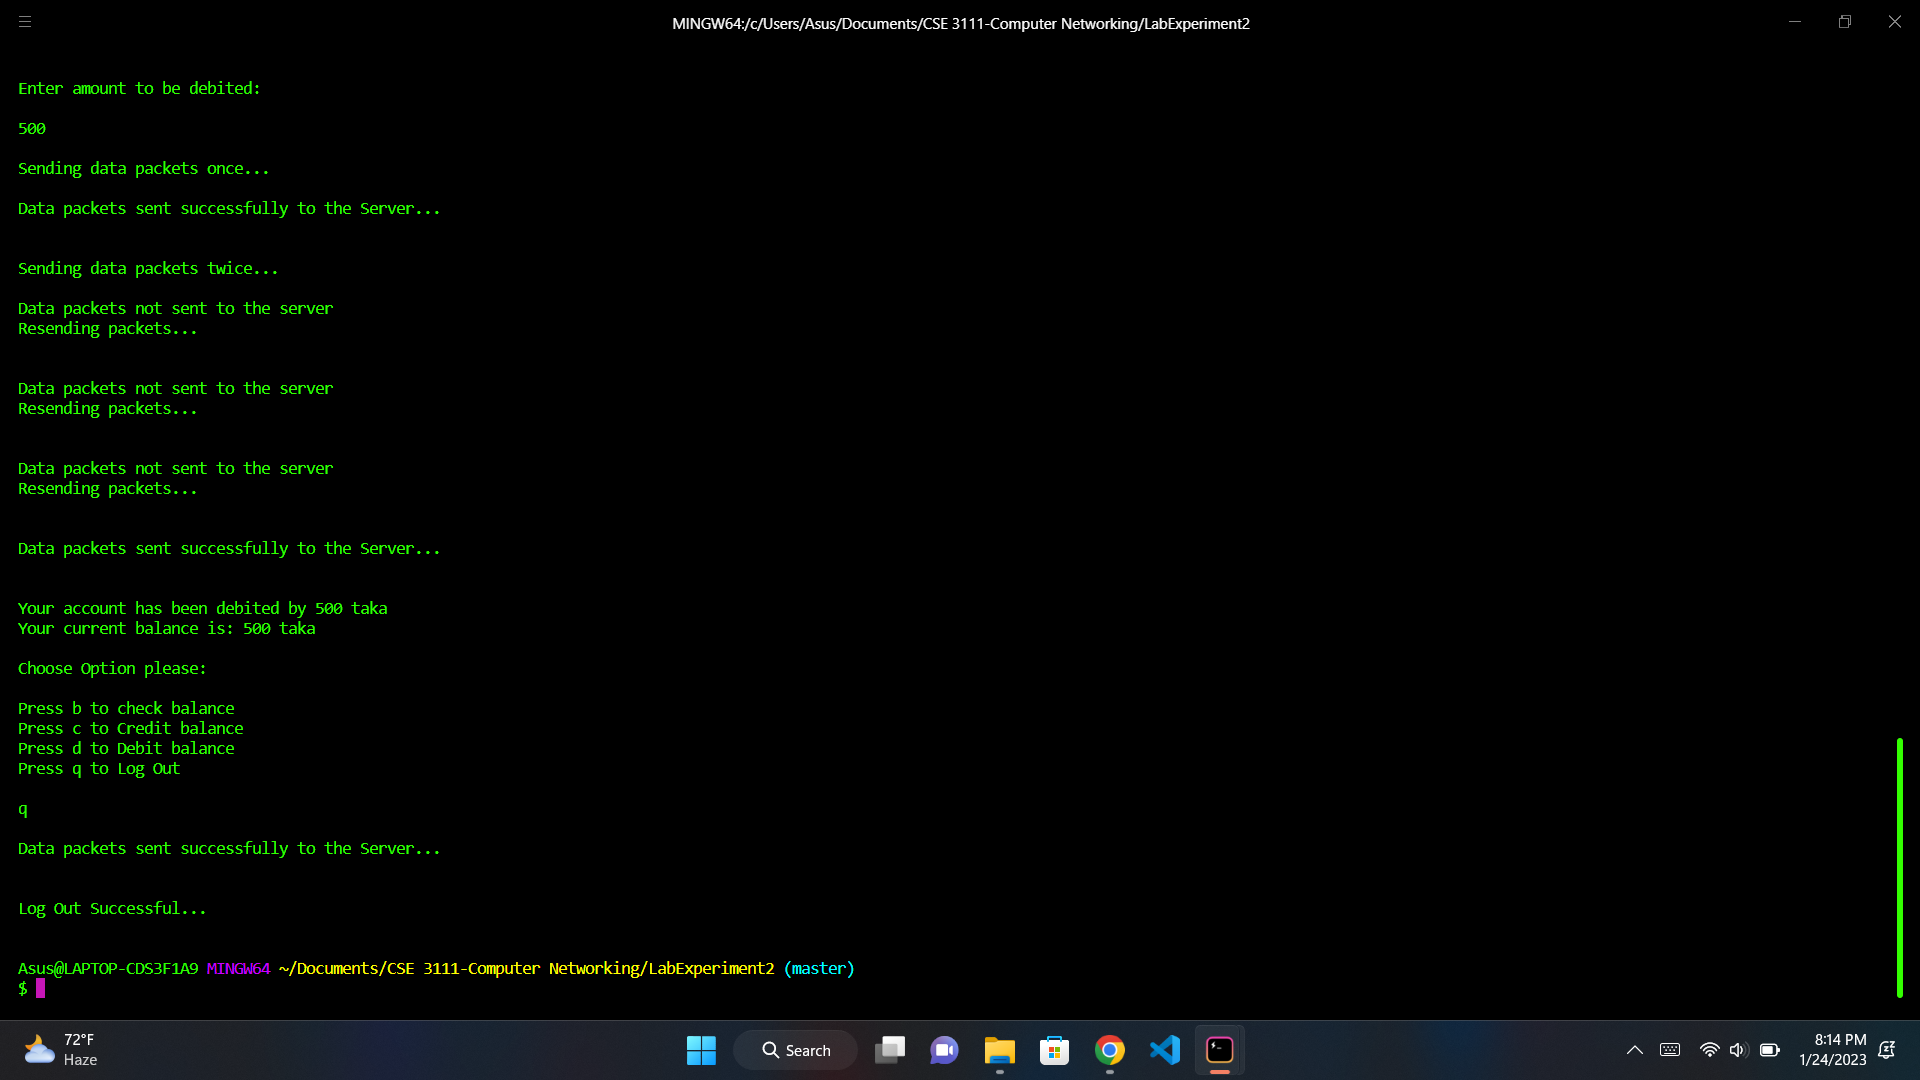
\includegraphics[width=\textwidth]{127.png}
\caption{User logs out}
\end{figure}


\begin{figure}[!h]
\centering
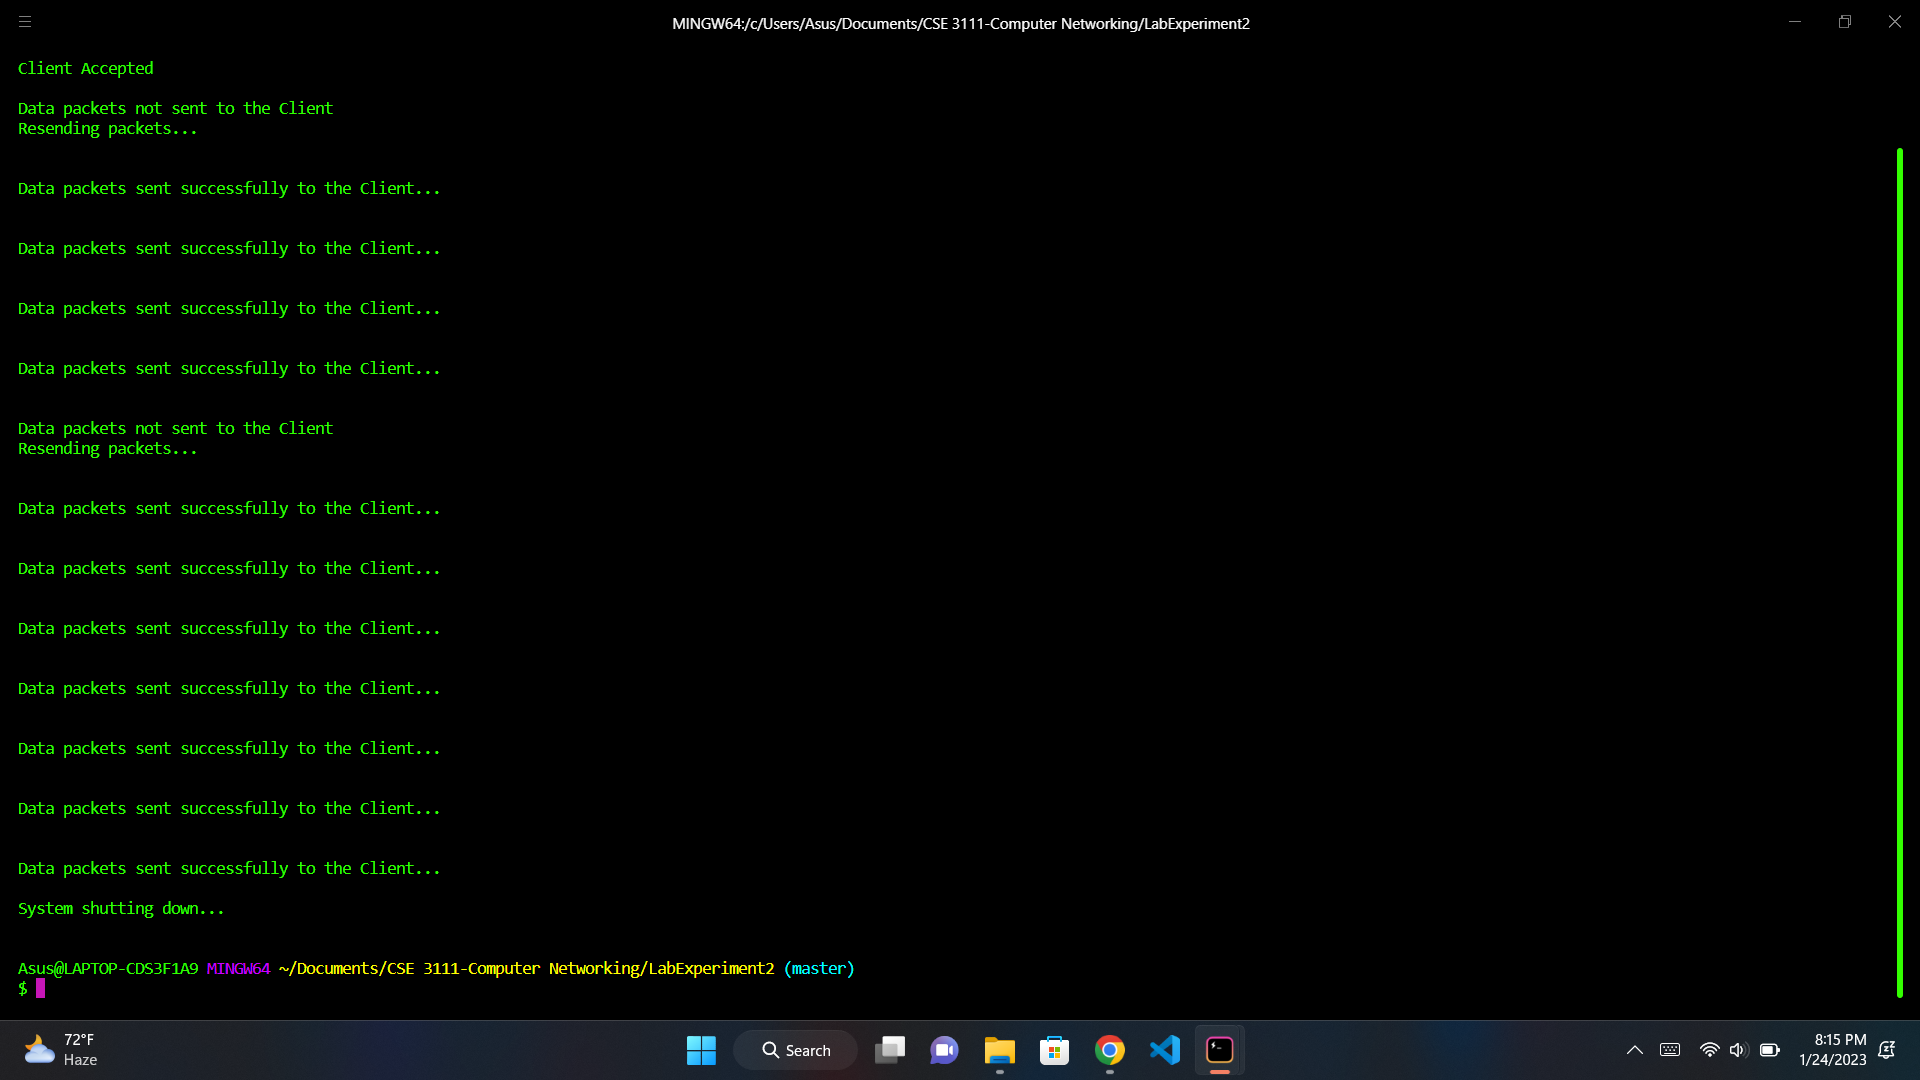
\includegraphics[width=\textwidth]{128.png}
\caption{System server shuts down}
\end{figure}

\newpage

\begin{figure}[!h]
\centering
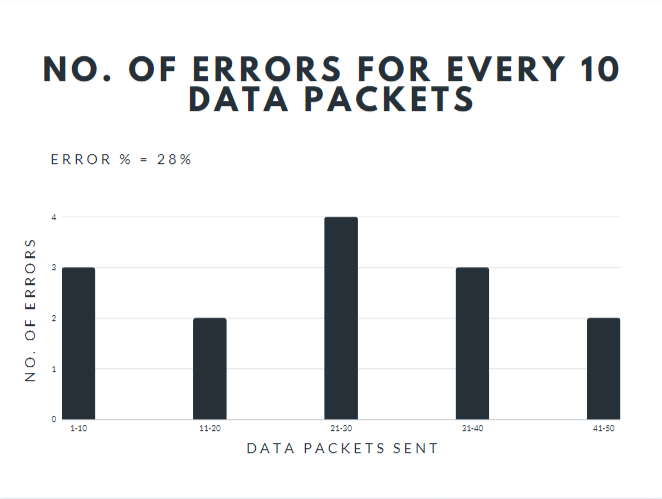
\includegraphics[width=\textwidth]{130}
\caption{ Error variation of data packet transmission}
\end{figure}











\newpage
\section{Experience}
\begin{enumerate}
\item We had to see some examples of how to use Socket Programming in Java
\item Write a simple program that creates a socket and uses it to send a message to a server and receive a response. 
\item Experiment with server and client interaction.
\item Write a simple program that creates a socket and uses it to send a message to a server and receive a response. 
\item Experiment with different types of sockets, such as TCP and UDP.
\item Learnt the principles of network programming, such as flow control, error handling, and security, and how they apply to socket programming.
\item Practice writing programs that use sockets to implement common network services such as a simple client-server or a file transfer program.
\end{enumerate}

\begin{thebibliography}{1}
\bibitem{book}  Computer networking : a top-down approach 6th ed.
\bibitem{StackOverflow} StackOverflow : \url{http://stackoverflow.com/}
\bibitem{Geeksforgeeks} Client-Server Application : 
\url{https://www.geeksforgeeks.org/establishing-the-two-way-communication-between-server-and-client-in-java/}
\end{thebibliography}

\end{document}